\documentclass[10pt,twocolumn]{article}

\usepackage[top=0.66in,bottom=0.70in,left=0.66in,right=0.66in]{geometry}
\usepackage[T1]{fontenc}
\usepackage[utf8]{inputenc}
\usepackage{lmodern}
\usepackage{microtype}
\usepackage{amsmath,amssymb,mathtools,bm}
\usepackage{graphicx}
\usepackage{booktabs,tabularx,array,multirow}
\usepackage{siunitx}
\usepackage{xcolor}
\usepackage{caption}
\usepackage{subcaption}
\usepackage{enumitem}
\usepackage{placeins}
\usepackage{float}
\usepackage{balance}
\usepackage{natbib}
\usepackage[hidelinks]{hyperref}

\graphicspath{{figures/}}
\sisetup{detect-all,round-mode=places,round-precision=4}
\newcolumntype{Y}{>{\raggedright\arraybackslash}X}
\newcolumntype{P}[1]{>{\raggedright\arraybackslash}p{#1}}
\newcommand{\method}{CSE-DKAN-FV}
\newcommand{\fixed}{fixed MC}
\newcommand{\todoauthor}[1]{\textcolor{red!70!black}{[AUTHOR ACTION: #1]}}
\setlength{\parindent}{1.2em}
\setlength{\parskip}{0.10em}
\setlength{\columnsep}{0.24in}
\setlength{\tabcolsep}{3.8pt}
\setlength{\emergencystretch}{1.5em}
\renewcommand{\arraystretch}{1.12}
\captionsetup{font=footnotesize,labelfont=bf}
\renewcommand{\topfraction}{0.95}
\renewcommand{\bottomfraction}{0.90}
\renewcommand{\textfraction}{0.05}
\renewcommand{\floatpagefraction}{0.82}
\setlength{\textfloatsep}{10pt plus 2pt minus 2pt}
\setlength{\floatsep}{9pt plus 2pt minus 2pt}
\makeatletter
\setlength{\@fptop}{0pt}
\setlength{\@fpsep}{10pt}
\setlength{\@fpbot}{0pt plus 1fil}
\makeatother

\title{Discontinuity-Aware KANs for Conservative Subcell Reconstruction of One-Dimensional Shocks}
\author{Jiakang Cao$^{1}$, Ze Tao$^{1}$, and Fujun Liu$^{1,*}$\\
\small $^{1}$School of Physics, Changchun University of Science and Technology,\\
\small Changchun, Jilin, China\\
\small $^{*}$Corresponding author: \href{mailto:waasledainbu776@gmail.com}{waasledainbu776@gmail.com}}
\date{}

\begin{document}
\maketitle

\begin{abstract}
Neural shock solvers often entangle two tasks: advancing conserved quantities and representing unresolved fronts. This coupling makes sharper reconstruction compete with conservation and admissibility. We test a narrower hypothesis: learning is more reliable when confined to the null space of the parent-cell averaging operator. The resulting \method{} solver advances cell averages with fixed Godunov or HLLC fluxes and uses a discontinuity-aware Kolmogorov--Arnold network (DKAN) only to redistribute each average among bounded subcells. Every learned correction has zero mean and is contracted toward fixed MC when an admissibility check fails. On preregistered ten-seed Burgers and Euler suites, the matched cross-equation error gain over fixed MC was 1.4259 (bootstrap 95\% confidence interval [1.3952, 1.4523]), above the predeclared 1.20 threshold. A frozen eight-case Euler suite then tested contacts, expansions, compression, shock--entropy interaction, wall reflections, and smooth advection. The learned reconstruction improved five of eight same-backbone comparisons, with a geometric-mean gain of 1.0429. It preserved parent means to $2.3\times10^{-13}$ and maintained positive density and pressure. A 512-cell HLLC solve remained more accurate in every case. The evidence therefore supports selective coarse-grid reconstruction, not a neural replacement for conservative evolution or grid refinement.
\end{abstract}

\noindent\textbf{Keywords:} physics-informed learning; Kolmogorov--Arnold networks; finite volume; shock capturing; Burgers equation; Euler equations; conservative machine learning

\section{Introduction}

Hyperbolic conservation laws govern compressible flow, hydraulic transients, traffic waves, and other systems with propagating fronts. Their physically relevant weak solutions can develop shocks from smooth initial data. A useful numerical approximation must therefore localize narrow transitions without losing conservation, admissibility, or the correct entropy solution \citep{leveque2002finitevolume,toro2009riemann}.

Physics-informed neural networks (PINNs) represent the solution as a differentiable field and optimize equation, initial, and boundary residuals \citep{raissi2019pinn}. This formulation is attractive for inverse problems and sparse observations. It is fragile at shocks because the classical differential form does not hold on the discontinuity, while composite losses can be ill conditioned \citep{wang2021gradient,krishnapriyan2021failure}. Weak-form, control-volume, entropy-aware, and artificial-viscosity formulations reduce this mismatch \citep{patel2022thermodynamic,coutinho2023avpinn,deryck2024wpinn}. In most cases, however, conservation and admissibility remain objectives to optimize rather than invariants of the hypothesis class.

Kolmogorov--Arnold networks (KANs) replace fixed node activations with trainable edge functions \citep{liu2024kan}. Fourier features enrich high-frequency representation \citep{zhang2025kaf}, while dynamic hyperbolic tangents provide a compact saturating response \citep{zhu2025dyt}. Lei, Exposito, and Mao used these ideas to construct a discontinuity-aware KAN-based PINN with mesh transformation and learnable local artificial viscosity \citep{lei2026dkanpinn}. Their results show that a stronger field approximator can sharpen shocks. They do not resolve a different question: what should the network be allowed to change when conservation must hold independently of optimization?

We address this question by restricting the learned hypothesis class. A classical finite-volume operator advances the parent-cell averages, while DKAN acts only on zero-mean subcell corrections. The network can therefore change the observed position and width of a front inside a parent cell, but it cannot alter the parent-grid trajectory. This differs from learning a solution field, a numerical flux, or a time-update rule. It is related to learned discretizations and conservative neural finite-volume schemes, but imposes a narrower role on learning \citep{barsinai2019discretization,kochkov2021cfd,lichtle2025unfv,cassia2024godunovloss,huang2025tvd}.

The contribution is this restriction of what is learned, rather than the juxtaposition of individually familiar numerical devices. Shared fluxes, zero-mean bases, deterministic sensing, and a posteriori rejection all implement one separation of responsibilities: the finite-volume scheme owns conservative evolution, and DKAN proposes only unresolved within-cell structure. This formulation creates a controlled same-backbone experiment because learned and fixed reconstructions share identical evolved averages. It also makes abstention testable on expansions, contacts, smooth waves, and under-resolved interactions. We evaluate these consequences against pointwise PINNs, direct DKAN-PINN, neural operators, and coarse- and fine-grid finite-volume baselines. The claims are limited to one-dimensional Burgers and ideal-gas Euler equations; no multidimensional generalization is asserted.

\section{Related work}

\subsection{PINNs for shocks}

Standard PINNs use a smooth neural approximation and strong residuals \citep{raissi2019pinn}. Gradient reweighting addresses competing loss scales but does not change the weak-solution mismatch \citep{wang2021gradient}. Adaptive localized artificial viscosity regularizes steep gradients \citep{coutinho2023avpinn}. Control-volume and thermodynamic losses improve balance and entropy behavior \citep{patel2022thermodynamic}. Weak PINNs instead test the conservation law against compactly supported functions and can approximate entropy solutions without differentiating through a shock \citep{deryck2024wpinn}. Our canonical comparisons include representative strong, gradient-weighted, artificial-viscosity, and coupled integral-loss variants.

DKAN-PINN targets representation rather than discrete conservation. Its adaptive Fourier embedding and edge-wise spline plus dynamic-tanh activation can fit sharper transitions than a conventional MLP \citep{lei2026dkanpinn}. Our canonical study reproduces this representational benefit while showing that lower field error need not reduce mass drift. The result separates the value of the DKAN parameterization from the conservation claim made here.

\subsection{Shock-capturing finite-volume methods}

Finite-volume schemes evolve cell averages using one shared numerical flux at each interface. Conservation follows from telescoping flux differences. HLLC restores the contact wave within the HLL family \citep{toro1994hllc}. ENO and WENO methods raise spatial order without accepting large oscillations near discontinuities \citep{jiang1996weno,borges2008wenoz}. Mean-preserving reconstruction and convex positivity limiting are established numerical principles \citep{zhang2010positivitydg,zhang2012positivityweno}. We use these principles to delimit the learned correction rather than claiming a new limiter theorem. WENO and exact Riemann solutions provide reference data, not additional trainable competitors.

\subsection{Learned solvers and neural operators}

Neural operators learn mappings between functions and amortize inference over problem families \citep{lu2021deeponet,li2021fno}. PDEBench provides standardized operator-learning tasks and metrics \citep{takamoto2022pdebench}. Learned discretizations can improve coarse-grid accuracy while retaining a classical stencil \citep{barsinai2019discretization,kochkov2021cfd}. Neural finite-volume methods have learned fluxes, update rules, or TVD limiters inside the evolution operator \citep{lichtle2025unfv,huang2025tvd}. Godunov-loss models instead embed approximate Riemann fluxes in the objective \citep{cassia2024godunovloss}. In contrast, our learned map is downstream of a frozen parent-cell update. It redistributes a known conservative average for output reconstruction and cannot change the shared interface flux.

\section{Governing equations and evaluation problems}

\subsection{Burgers equation}

We consider the scalar equation
\begin{equation}
  u_t + \left(\frac{u^2}{2}\right)_x = \nu u_{xx},
  \qquad x\in[-1,1],
  \label{eq:burgers}
\end{equation}
with periodic boundaries and
\begin{equation}
  u(x,0)=\bar u-A\sin(\pi x).
\end{equation}
The canonical test uses $\bar u=0.2$, $A=1$, $\nu=0$, and $t_f=0.6$. The frozen family varies $A$ over ten values from 0.27 to 2.94 and $\nu$ over $\{0,10^{-4},3\times10^{-4},10^{-3},3\times10^{-3},10^{-2}\}$. References use adaptive high-resolution WENO with 1024--4096 cells, depending on viscosity.

\subsection{Compressible Euler equations}

The one-dimensional ideal-gas Euler equations are
\begin{equation}
 \bm U_t+\bm F(\bm U)_x=0,
 \quad
 \bm U=
 \begin{bmatrix}\rho\\ \rho u\\ E\end{bmatrix},
 \quad
 \bm F=
 \begin{bmatrix}\rho u\\ \rho u^2+p\\ u(E+p)\end{bmatrix},
 \label{eq:euler}
\end{equation}
where $p=(\gamma-1)(E-\rho u^2/2)$ and $\gamma=1.4$. The canonical Sod problem uses $(\rho,u,p)_L=(1,0,1)$ and $(\rho,u,p)_R=(0.125,0,0.1)$ at $t_f=0.2$ \citep{sod1978survey}. The frozen validation uses ten unseen Riemann problems at 100, 200, and 400 parent cells. The engineering extension contains 20 in-distribution and ten stress cases. A separate mechanism suite adds the Lax tube \citep{lax1954weak}, an isolated contact, double rarefaction, colliding streams, Shu--Osher shock--entropy interaction \citep{shu1989eno2}, Woodward--Colella interacting blast waves \citep{woodward1984strongshocks}, and smooth periodic entropy-wave advection. Exact solutions are used when available; otherwise independently refined HLLC trajectories define the reference.

\section{Conservative learning as a null-space reconstruction}

\subsection{Design principle: the update is fixed}

Let $\mathcal A$ denote the averaging operator over $Q$ subcells. We restrict every learned correction $\delta\bm U_{\theta,i,q}$ to its null space:
\begin{equation}
 \bm U_{i,q}=\bar{\bm U}_i+\delta\bm U_{\theta,i,q},
 \qquad
 \mathcal A(\delta\bm U_{\theta,i})
 =\frac{1}{Q}\sum_{q=1}^{Q}\delta\bm U_{\theta,i,q}=\bm 0.
 \label{eq:nullspace}
\end{equation}
The finite-volume solver determines $\bar{\bm U}_i$, and DKAN proposes only its within-cell distribution. This restriction is the model identity. It prevents the learned map from changing the evolved parent means, irrespective of training loss or checkpoint quality.

Figure~\ref{fig:architecture} follows this separation from supervision to deployment. Exact or WENO records define an oracle subcell blend, but backpropagation updates only the DKAN gate. At inference, the frozen gate acts after the Godunov or HLLC evolution. A posteriori checks accept the proposed profile or contract it toward fixed MC. The model is therefore not a pointwise PINN, and no MLP performs the trainable reconstruction role. HLLC supplies the Euler dissipation; entropy is audited rather than optimized or guaranteed.

\begin{figure*}[t]
  \centering
  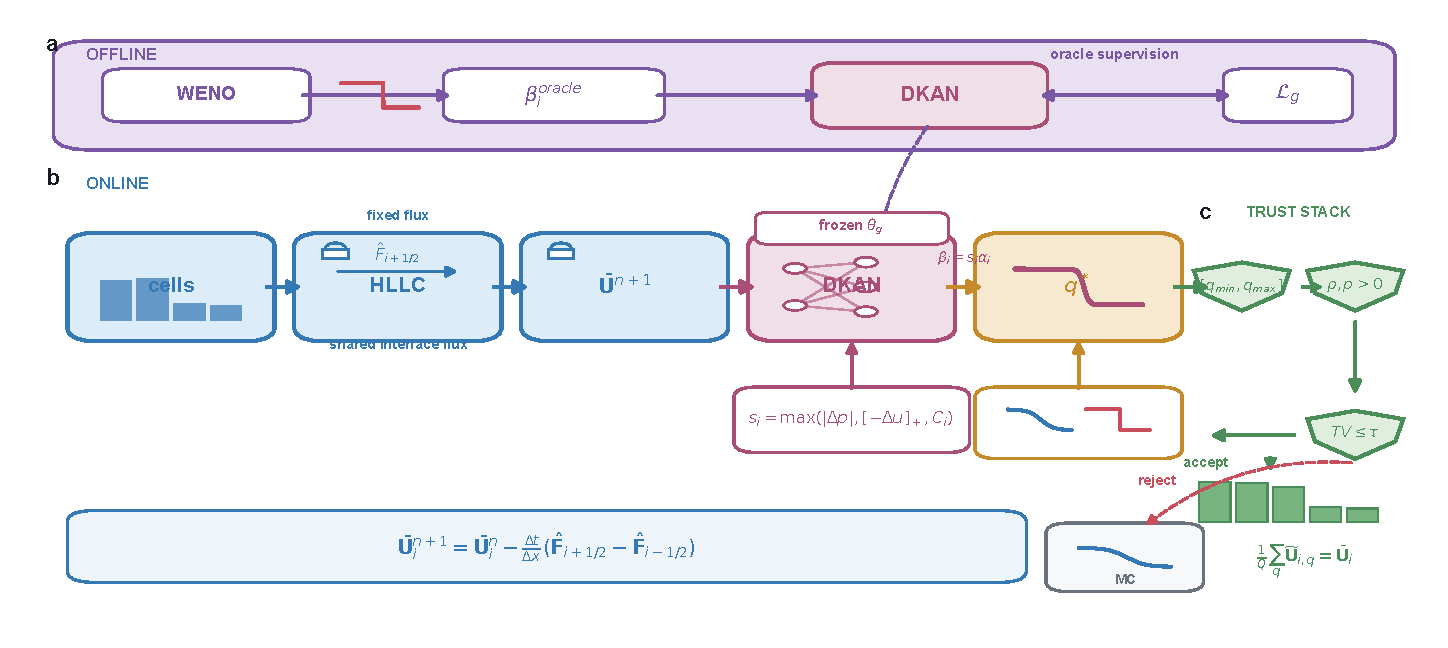
\includegraphics[width=\textwidth]{fig1_cse_dkan_fv_architecture.pdf}
  \caption{Division of responsibility in \method{}. \textbf{a}, Exact or WENO records supervise only the DKAN gate. \textbf{b}, Shared HLLC fluxes determine the parent-cell trajectory, after which the frozen gate proposes a zero-mean MC--jump reconstruction. \textbf{c}, A posteriori tests accept the proposal or contract it toward fixed MC. Every admissible point on this path preserves the evolved parent mean; curves and cell glyphs are schematic.}
  \label{fig:architecture}
\end{figure*}

\subsection{Fixed parent-cell evolution}

For a parent cell $I_i$, the state average evolves as
\begin{equation}
 \bar{\bm U}_i^{n+1}=\bar{\bm U}_i^n
 -\frac{\Delta t}{\Delta x}
 \left(\widehat{\bm F}_{i+1/2}-\widehat{\bm F}_{i-1/2}\right).
 \label{eq:fv}
\end{equation}
Burgers uses the exact scalar Godunov flux and SSP-RK3 integration with Courant number 0.35. Euler uses HLLC with Davis outer-wave estimates, primitive-variable MC slopes, SSP-RK3, and Courant number 0.25. Primitive slopes are scaled when an interface state would violate the density or pressure floor.

\subsection{DKAN parameterization of the conservative correction}

Each DKAN edge combines a dynamic-tanh atom with a cubic B-spline expansion. For input $z_i$ and output channel $j$, the edge function is
\begin{equation}
 \phi_{ji}(z_i)=w^{(d)}_{ji}\tanh\!\left(a_{ji}(z_i-b_{ji})\right)
 +s_{ji}\sum_{k=1}^{K}c_{jik}B_k(z_i).
 \label{eq:dkan}
\end{equation}
The slope satisfies $a_{ji}>0$ through a softplus parameterization. We use five spline intervals and cubic splines. This implementation follows the structural DKAN equation in Ref.~\citep{lei2026dkanpinn}, while adapting the input and output roles to finite-volume reconstruction.

Figures~\ref{fig:encoder} and \ref{fig:dkanmechanism} separate the learned proposal from its conservative realization. DKAN no longer maps $(x,t)$ to a global flow field. It maps a local stencil to the bounded coefficient $\alpha_i$. Localized jump responses and smooth spline responses share the same edge-wise graph, so the network represents how strongly a mean-preserving candidate should depart from fixed MC. A deterministic sensor then forms $\beta_i=s_i\alpha_i$. In the schematics, $s_i$ denotes the Burgers jump--viscous gate or the Euler factor $\eta\chi_i$.

\begin{figure*}[t]
  \centering
  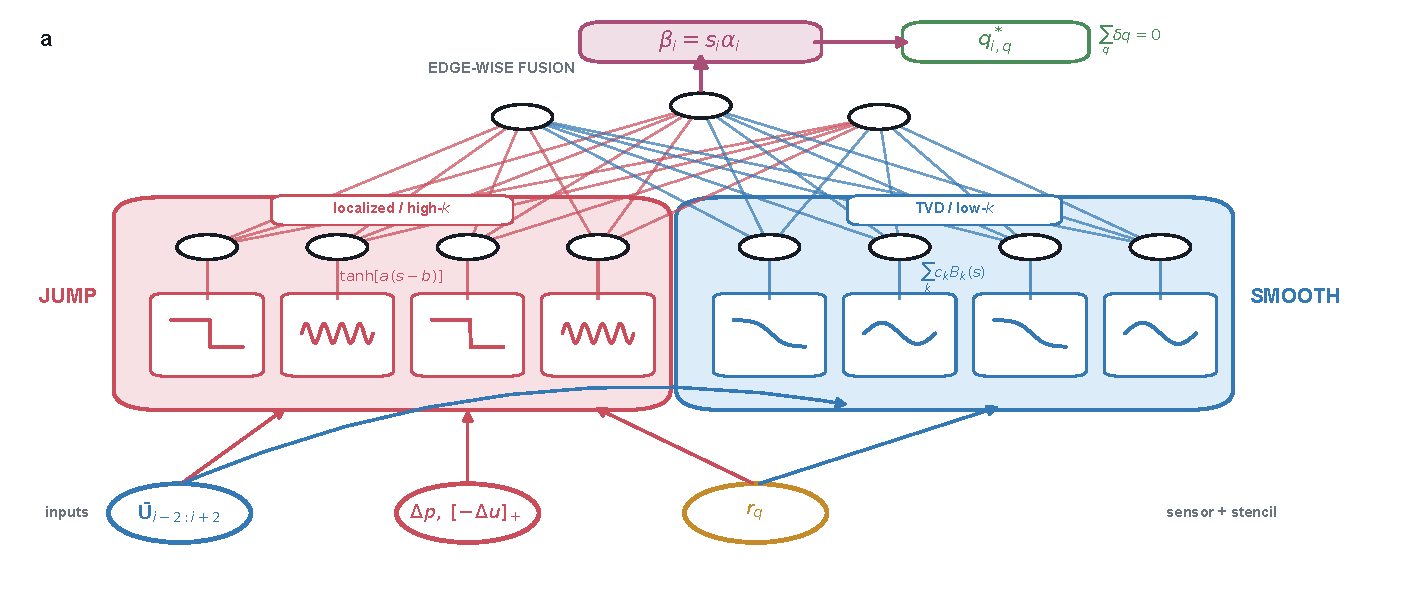
\includegraphics[width=\textwidth]{fig2_multiscale_feature_encoder.pdf}
  \caption{Local evidence used to parameterize a conservative correction. Stencil states and compression indicators excite localized tanh and smooth spline responses. Edge-wise fusion returns $\alpha_i$, while the deterministic sensor forms $\beta_i=s_i\alpha_i$. The coefficient scales a zero-mean candidate rather than a new time update; curves are schematic basis responses.}
  \label{fig:encoder}
\end{figure*}

Figure~\ref{fig:dkanmechanism} resolves the edge map and the induced correction. Each edge combines a localized dynamic-tanh atom with a cubic B-spline expansion. The sensor modulates the learned gate before fixed MC and explicit jump profiles are blended. Because both profiles share the same average, every admissible blend satisfies Eq.~\eqref{eq:nullspace}.

\begin{figure*}[t]
  \centering
  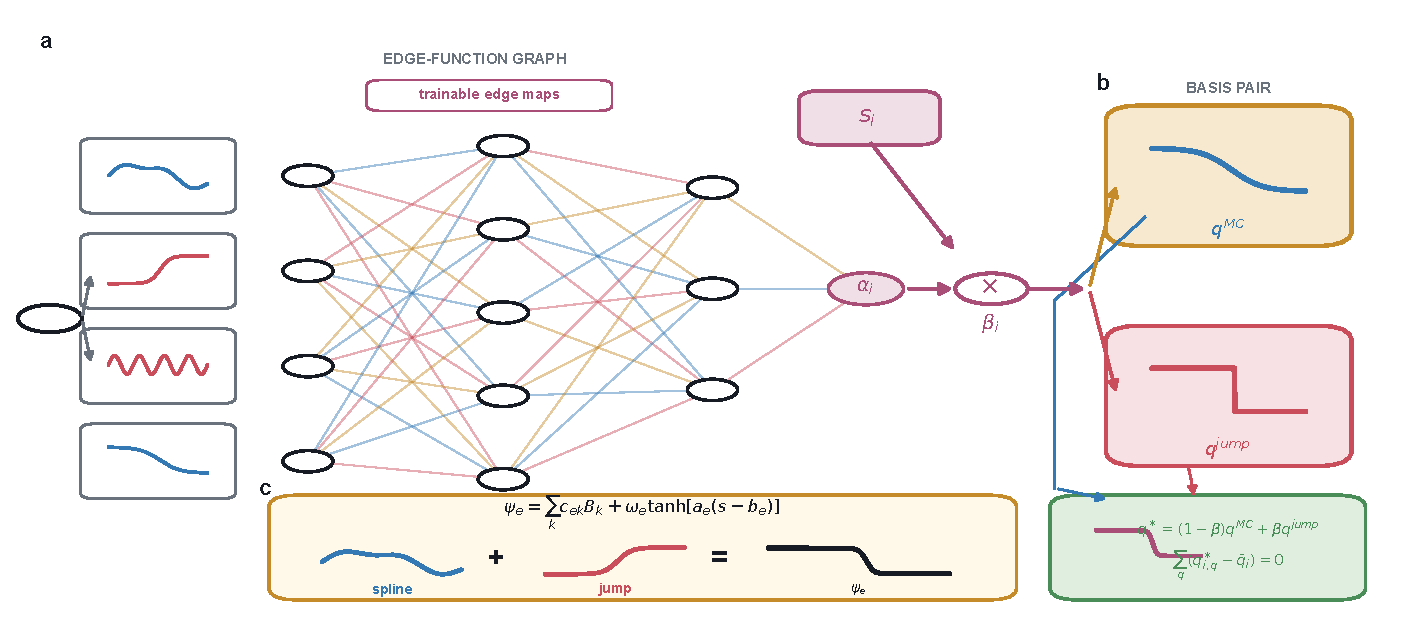
\includegraphics[width=\textwidth]{fig3_dkan_edge_subcell.pdf}
  \caption{From a DKAN gate to a mean-preserving profile. \textbf{a}, Edge-specific functions map local features to $\alpha_i$. \textbf{b}, The sensor forms $\beta_i$ and interpolates between MC and jump profiles with the same parent mean. \textbf{c}, Each edge combines cubic B-splines with a localized dynamic-tanh atom. The output changes subcell placement but remains in the averaging null space; curves are schematic.}
  \label{fig:dkanmechanism}
\end{figure*}

\subsection{Scalar realization: Burgers equation}

Let $\xi_q\in(-1/2,1/2)$ denote $Q$ symmetric subcell coordinates, with $\sum_q\xi_q=0$. The reconstructed scalar profile is
\begin{equation}
 u_{i,q}=\bar u_i+\theta_i\left[
 m_i\xi_q+\lambda_i s_i\left(r_{i,q}-\frac{1}{Q}\sum_{q'=1}^{Q}r_{i,q'}\right)
 \right].
 \label{eq:burgers_recon}
\end{equation}
Here, $m_i$ is the MC slope, $s_i$ is a local variation scale, and $r_{i,q}$ is the DKAN output. The zero-mean terms imply $Q^{-1}\sum_q u_{i,q}=\bar u_i$ before and after convex scaling.

The multiplier $\lambda_i$ combines two gates. A normalized five-cell jump sensor activates the learned residual only near a sufficiently large interface jump. A viscous-width gate disables the discontinuous expert when
\begin{equation}
 \frac{8\,\operatorname{atanh}(0.8)\nu}{\Delta u_i\,\Delta x}>2,
 \label{eq:viscousgate}
\end{equation}
because the analytic 10--90\% travelling-wave thickness already spans more than two parent cells. This gate is analytic, not a learned artificial viscosity. The scalar $\theta_i\in[0,1]$ keeps every subcell value inside the five-cell stencil range. A final conservative convex projection restricts total variation to 5\% above its declared reference budget in the frozen Burgers protocol.

\subsection{System realization: Euler equations}

Euler reconstruction uses four subcells in the engineering study and eight in the frozen validation. A fixed conservative MC profile $\bm U^{\mathrm{MC}}_{i,q}$ is blended with an explicit conservative jump profile $\bm U^{\mathrm{jump}}_{i,q}$:
\begin{equation}
 \bm U_{i,q}=\bm U^{\mathrm{MC}}_{i,q}
 +\eta\alpha_i\left(\bm U^{\mathrm{jump}}_{i,q}-\bm U^{\mathrm{MC}}_{i,q}\right),
 \qquad \alpha_i=\sigma\!\left(g_{\theta}(\bm z_i)\right).
 \label{eq:eulerblend}
\end{equation}
The DKAN $g_{\theta}$ receives 12 normalized conservative-variable differences from a five-cell stencil and three primitive context variables. These are $\tanh(\log\rho)$, $\tanh(u/c)$, and $\tanh(\log p)$. The global trust factor is $\eta=0.75$ in the frozen protocol. In the mechanism-diverse protocol, the effective blend is $\eta\alpha_i\chi_i$, where $\chi_i$ is an explicit local discontinuity sensor. With $R(z;a,b)=\operatorname{clip}[(z-a)/(b-a),0,1]$, normalized pressure jump $J_p$, normalized density jump $J_\rho$, and compressive velocity indicator $C_u$, we use
\begin{equation}
\begin{aligned}
 \chi_i=\max\!\bigl\{&R(J_p;0.025,0.15),
 R(C_u;0.02,0.15),\\
 &R(J_\rho;0.15,0.35)\bigr\}.
\end{aligned}
 \label{eq:eulersensor}
\end{equation}
The higher density-only threshold admits isolated contacts while rejecting resolved smooth entropy waves. The thresholds and combination rule were fixed before the final sensor-enabled evaluation, and no neural checkpoint was retrained.

The jump basis and fixed MC basis share the parent-cell conservative mean. A componentwise stencil limiter then scales the complete correction. A 32-step bisection finds the largest convex multiplier that maintains $\rho\ge10^{-8}$ and $p\ge10^{-8}$. The 400-cell frozen cases fall back to fixed MC because the learned correction was calibrated only through 200 cells.

The engineering diagnostic adds a global density-TV projection. Given fixed and candidate profiles, it finds the largest $\beta\in[0,1]$ such that
\begin{equation}
 \begin{aligned}
 \operatorname{TV}_{\rho}\!\bigl(&\bm U^{\mathrm{MC}}+
 \beta(\bm U^{\mathrm{cand}}-\bm U^{\mathrm{MC}})\bigr)\\
 &\le (1+\delta)\operatorname{TV}_{\rho}(\bm U^{\mathrm{MC}})+10^{-12}.
 \end{aligned}
 \label{eq:tvprojection}
\end{equation}
We report $\delta\in\{0,0.02,0.05,0.10\}$ and the unprojected model. The 2\% setting was registered after the main engineering benchmark and is therefore a diagnostic, not part of its original accuracy gate.

Panel \textbf{c} of Fig.~\ref{fig:architecture} distinguishes three evidence levels. Shared interface fluxes and Eq.~\eqref{eq:nullspace} give algebraic conservation. Stencil bounds and positivity are deterministic acceptance tests. Density TV further restricts deployment but does not alter the finite-volume update. Entropy, Rankine--Hugoniot consistency, shock width, and runtime remain empirical audits rather than mathematical guarantees.

\subsection{Offline supervision and frozen deployment}

All DKAN subcell models are supervised by high-resolution WENO or exact Riemann data. The frozen protocols use ten independently initialized float64 checkpoints. The Burgers model learns from local subcell targets across amplitude and viscosity. The Euler model learns a scalar blend between fixed MC and the jump basis. Validation checkpoint selection precedes the blind evaluation.

For an Euler training record $r$, the oracle blend $\alpha_r^\star$ minimizes the local profile mismatch between the two bases and the reference. The optimized objective is a weighted oracle loss
\begin{equation}
 \mathcal L_{\mathrm{gate}}=
 \frac{\sum_r w_r\left[\sigma(g_\theta(\bm z_r))-\alpha_r^\star\right]^2}
 {\sum_r w_r},
 \label{eq:gateloss}
\end{equation}
where $w_r$ emphasizes informative discontinuity records. The selected checkpoint minimizes held-out primitive-profile mean-squared error after all hard projections. FNO minimizes a spatially weighted primitive-field MSE on the parameterized Riemann family.

The engineering Euler model uses 64 training cases, 64 and 128 parent cells, four subcells, and times 0.08, 0.16, and 0.28. Three float64 seeds are trained for 2500 iterations with batches of 1024 local stencils. The complete engineering model has 6284 parameters, including 3089 trainable DKAN gate parameters. The FNO uses 512 training and 128 validation cases sampled from the declared range. It operates on 512 points with width 32, 24 Fourier modes, four layers, 2000 iterations, and three float32 seeds. Its parameter count is 105027.

\section{Experimental design}

\subsection{Comparators}

The canonical study compares MLP-PINN, gradient-weighted PINN (GW-PINN), artificial-viscosity PINN (AV-PINN), coupled integral PINN (CI-PINN), direct DKAN-PINN, fixed finite-volume reconstruction, and \method{}. All four MLP-based PINNs share the same architecture within each equation. Burgers models have 8641 optimized parameters, while Euler models have 8707. The direct DKAN-PINN uses the DKAN field architecture but retains pointwise residual training. WENO and exact Riemann solutions define reference values rather than additional learned rows.

The engineering study compares a PDEBench-style FNO, 128-cell HLLC with piecewise-constant or fixed MC output, two DKAN-FV training distributions, and 512-cell HLLC. The fine-grid method is an accuracy--cost reference. The proposed method is not required to beat a four-times-finer conservative solve.

\subsection{Metrics and statistical units}

For a field $v$, normalized error is
\begin{equation}
 E_v=\frac{\lVert v-v^\star\rVert_2}{\lVert v^\star\rVert_2+10^{-12}}.
\end{equation}
The canonical and 30-case studies retain the preregistered geometric state error $E_{\mathrm{geo}}=(E_\rho E_u E_p)^{1/3}$. For the mechanism suite, the primary score is instead
\begin{equation}
 E_{\mathrm{RMS}}=\left[\frac{E_\rho^2+E_u^2+E_p^2}{3}\right]^{1/2}.
 \label{eq:rmsmetric}
\end{equation}
This amendment was frozen after an implementation smoke test and before the formal eight-case run because $E_{\mathrm{geo}}$ degenerates on an isolated contact, whose exact velocity and pressure errors are near machine precision. Error gain is $G=E_{\mathrm{baseline}}/E_{\mathrm{model}}$, so $G>1$ favors the new model. Shock width is the distance between 10\% and 90\% levels on a detected monotone jump.

For the detailed mechanism plates, Eq.~\eqref{eq:rmsmetric} is evaluated at intermediate physical times,
\begin{equation}
 \mathcal L_{\mathrm{case}}(t)=
 \left\{\frac{1}{3}\sum_{v\in\{\rho,u,p\}}
 \left[\frac{\lVert \widehat v(\cdot,t)-v^\star(\cdot,t)\rVert_2}
 {\lVert v^\star(\cdot,t)\rVert_2+10^{-12}}\right]^2\right\}^{1/2}.
 \label{eq:caseloss}
\end{equation}
This is a time-resolved \emph{evaluation} loss, not a per-case training loss. The FNO and both DKAN gates were trained once on problem families, so assigning a separate optimization history to each held-out case would be methodologically incorrect.

Hard conservation is the maximum change between a parent-cell conservative mean and the mean of its reconstructed subcells. The Euler audit also records minimum density and pressure, domain-integral error, density-TV excess, entropy violation, and normalized Rankine--Hugoniot residual. Specific entropy is $s=\log(p/\rho^\gamma)$, with the shock orientation taken from the exact Riemann wave pattern.

The frozen Burgers statistic contains 600 seed--case pairs; Euler contains 300. These pairs are not treated as independent training replicates. We first aggregate each seed geometrically, then bootstrap the ten matched seed-level values. The cross-equation statistic is the geometric mean of matched Burgers and Euler seed gains.

\subsection{Per-case diagnostic protocol}

Each of the eight detailed Euler audits uses 13 equally spaced physical times from the initial state to $t_f$. At every nonzero time, the reference and all six deployed models are evaluated on the same 512 cell-centre coordinates. The 128-cell methods are expanded through piecewise-constant, fixed-MC, or DKAN subcell reconstruction; the fine comparator evolves 512 HLLC parent cells. Learned predictions are pointwise medians over three frozen seeds. No checkpoint is updated on an audited case.

Each case is represented once by a single integrated diagnostic plate. Its upper atlas assigns every model one predicted density field and one co-registered absolute-density-error field over $(x,t)$; density and logarithmic error scales are shared within the case, and reference contours are overlaid on every prediction. The supporting panels give the final density, velocity, and pressure profiles, $\mathcal L_{\mathrm{case}}(t)$, the effective sensor--DKAN gate $\chi\alpha$, and the final component-error matrix. The paired table reports all component errors, $E_{\mathrm{RMS}}$, density-TV excess, positivity minima, and online time. Parent-to-subcell mean preservation is reported separately because it is an algebraic property, not a reference-dependent field metric.

\subsection{Predeclared decision rules}

The strong frozen claim requires a median cross-equation gain of at least 1.20 and a bootstrap lower bound above 1.00. We additionally report whether the 95\% lower bound exceeds 1.20. The engineering same-backbone gate requires a paired median gain of at least 1.05 and a win rate of at least 60\%. The stress gate requires a median gain of at least 1.00 and a win rate of at least 50\%. Every claimed DKAN-FV output must preserve means within $10^{-12}$ and maintain positive density and pressure.

\section{Results}

\subsection{Validation loss does not predict transfer}

The FNO median training loss decreased from 2.360 to 0.03996, and its validation MSE decreased from 1.057 to 0.04571. The engineering DKAN profile MSE decreased from 0.004038 to 0.003353. The narrow Sod-neighbourhood DKAN reached 0.0007971 on its smaller validation distribution, yet transferred less reliably. Model selection loss therefore cannot rank deployment performance across different training distributions. FNO and both DKAN gates were trained once on families rather than fitted to each test. The case curves below are frozen time-resolved \emph{evaluation} losses from Eq.~\eqref{eq:caseloss}, not eight training histories.

\subsection{Generalization is mechanism-selective}

The eight cases were selected by physical mechanism before checkpoint evaluation. Sod and Lax vary the state regime, while the moving contact isolates a linearly degenerate wave. Double rarefaction stresses positivity, and colliding streams test symmetric compression. Shu--Osher and Woodward--Colella introduce interactions absent from training. Smooth periodic advection is a negative control for false activation. No case was removed after loss inspection. Figure~\ref{fig:mechanismoverview} shows the resulting coverage, and Table~\ref{tab:mechanismdefs} states the question assigned to each case.

\begin{figure*}[t]
 \centering
 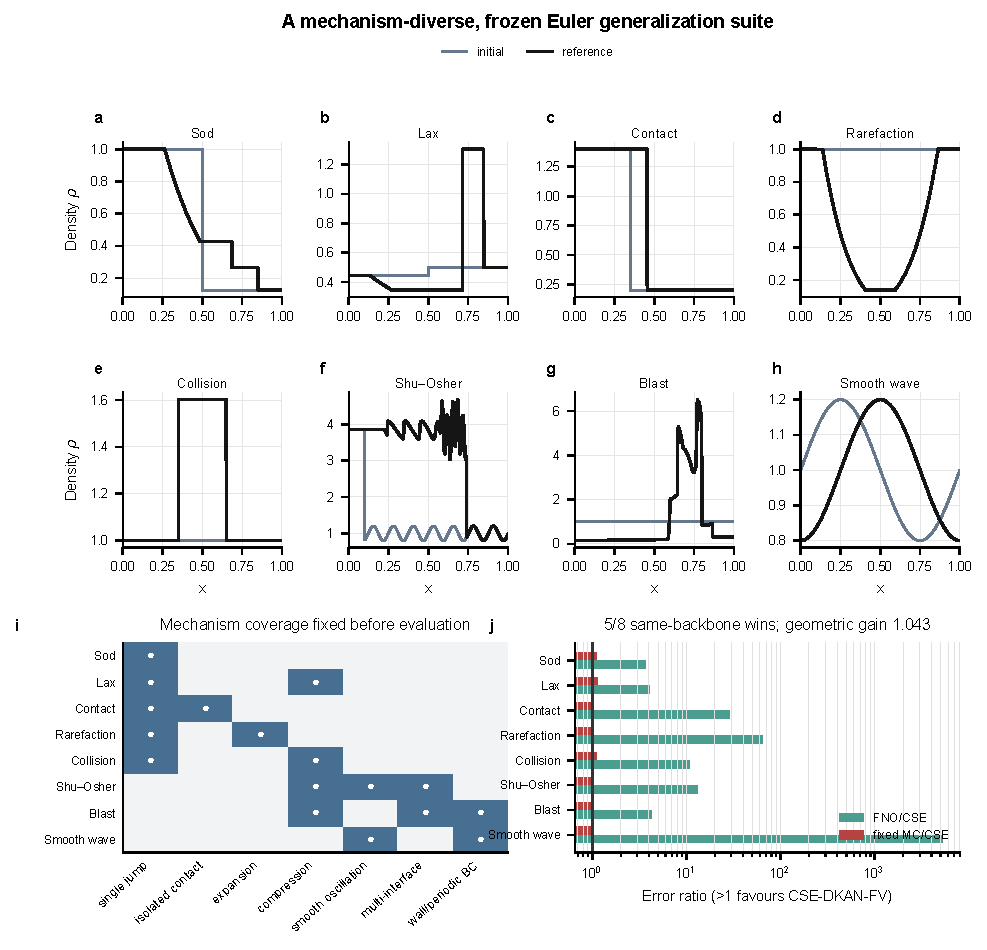
\includegraphics[width=\textwidth]{fig12_mechanism_suite_overview.pdf}
 \caption{Frozen mechanism-diverse Euler suite. \textbf{a--h}, Initial and final reference density profiles. \textbf{i}, Mechanism-coverage matrix fixed before evaluation. \textbf{j}, FNO/CSE and fixed-MC/CSE error ratios on the RMS metric; the vertical line marks parity. The proposed reconstruction wins five of eight same-backbone comparisons but the gain is generally modest, whereas the frozen FNO transfers poorly outside its training family.}
 \label{fig:mechanismoverview}
\end{figure*}

\begin{table*}[t]
\centering
\caption{Mechanism-diverse case definitions. Piecewise states are $(\rho,u,p)$. ``Analytic'' includes exact Riemann and periodic-advection solutions. Gains are final RMS baseline error divided by CSE error.}
\label{tab:mechanismdefs}
\scriptsize
\begin{tabularx}{\textwidth}{P{0.105\textwidth}P{0.26\textwidth}P{0.095\textwidth}P{0.29\textwidth}rr}
\toprule
Case & Initial data and boundary & $t_f$/reference & Generalization question & Fixed/CSE & FNO/CSE\\
\midrule
Sod & $(1,0,1)$; $(0.125,0,0.1)$, outflow & 0.20/analytic & Canonical rarefaction--contact--shock anchor & 1.120 & 3.686\\
Lax & $(0.445,0.698,3.528)$; $(0.5,0,0.571)$, outflow & 0.14/analytic & Stronger pressure and velocity regime & 1.127 & 4.019\\
Moving contact & $(1.4,0.35,1)$; $(0.2,0.35,1)$ at $x=0.35$ & 0.30/analytic & Isolated linearly-degenerate wave without a shock & 1.005 & 28.42\\
Double rarefaction & $(1,-1.5,0.6)$; $(1,1.5,0.6)$, outflow & 0.15/analytic & Expansion, low-density centre, and positivity & 0.999 & 63.98\\
Colliding streams & $(1,0.6,1)$; $(1,-0.6,1)$, outflow & 0.15/analytic & Compression-dominated two-shock formation & 1.099 & 10.86\\
Shu--Osher & $(3.857143,2.629369,10.33333)$ against $\rho=1+0.2\sin(50x-25)$, $u=0,p=1$ & 0.18/HLLC-2048 & Shock interacting with unseen smooth oscillations & 1.000 & 12.98\\
Woodward--Colella & $\rho=1,u=0$; $p=1000,0.01,100$ on $[0,0.1),[0.1,0.9),[0.9,1]$, reflecting & 0.038/HLLC-4096 & Multiple shocks, wall reflection, and extreme pressure ratio & 1.006 & 4.252\\
Smooth entropy & $\rho=1+0.2\sin(2\pi x)$, $u=p=1$, periodic & 0.25/analytic & Negative control for false discontinuity activation & 1.000 & 5220\\
\bottomrule
\end{tabularx}
\end{table*}

The proposed/fixed geometric-mean gain was 1.0429, and five of eight cases favored the learned reconstruction. The median gain was only 1.0053, which shows that the benefit was concentrated in selected compression cases. The frozen FNO had a 23.21-fold geometric error ratio relative to CSE, with a minimum case ratio of 3.686. This is an out-of-distribution result, not evidence of intrinsic FNO inferiority. CSE preserved parent-cell means to $2.27\times10^{-13}$ and maintained positive states. Its maximum density-TV ratio relative to fixed MC was 1.02053. The 512-cell HLLC comparator was more accurate in all eight cases.

\subsubsection{Sod: canonical three-wave anchor}

Sod anchors the new suite to the canonical rarefaction--contact--shock topology. CSE reduces RMS error from 0.04223 to 0.03770 (1.120-fold), primarily through velocity and pressure, while its effective gate remains localized (mean 0.00642; 1.56\% of final cells above 0.1). The narrow DKAN is slightly better at 0.03383, so this case does not by itself justify the broader engineering gate. Fine HLLC remains best at 0.02669.

The density atlas separates the three sources of error. All 128-cell conservative methods place the rarefaction and contact correctly at the parent-cell scale, but fixed MC spreads the right-moving shock over a wider subcell neighbourhood. CSE reduces the shock-aligned velocity and pressure bands without changing the parent trajectory. Its density error is not uniformly smaller: the narrow-family gate has the lowest aggregate score because its calibration is closest to Sod. This distinction prevents the canonical example from being used as circular evidence for broad generalization.

The temporal curve supports the same interpretation. CSE is better than fixed MC at nine of the twelve nonzero audit times. At the first recorded time their errors are 0.1129 and 0.1154; at $t_f$ they are 0.03770 and 0.04223. The gain therefore develops as the three waves separate, rather than being an initial-condition interpolation advantage. FNO decreases from 0.708 at the first audit to 0.139, but its spatial fields retain larger amplitude and front errors. The case shows that constrained reconstruction can help on its canonical topology. The narrow-model and fine-grid results delimit both the learned effect and the remaining resolution gap.

The computational comparison is similarly bounded. CSE adds 0.0249~s to the 0.6909~s coarse HLLC evolution, whereas increasing the parent grid to 512 cells costs 3.292~s. Thus, the learned observation map recovers some profile accuracy at small incremental cost, but it cannot correct evolution error already embedded in the shared 128-cell averages. This separation explains why the CSE and fixed rows have identical positivity minima yet different subcell errors. It also clarifies the role of the canonical test in the paper: Sod confirms that replacing the trainable reconstruction by DKAN is operational, while the remaining seven cases determine whether that replacement is selective and transferable.

\begin{figure*}[p]
 \centering
 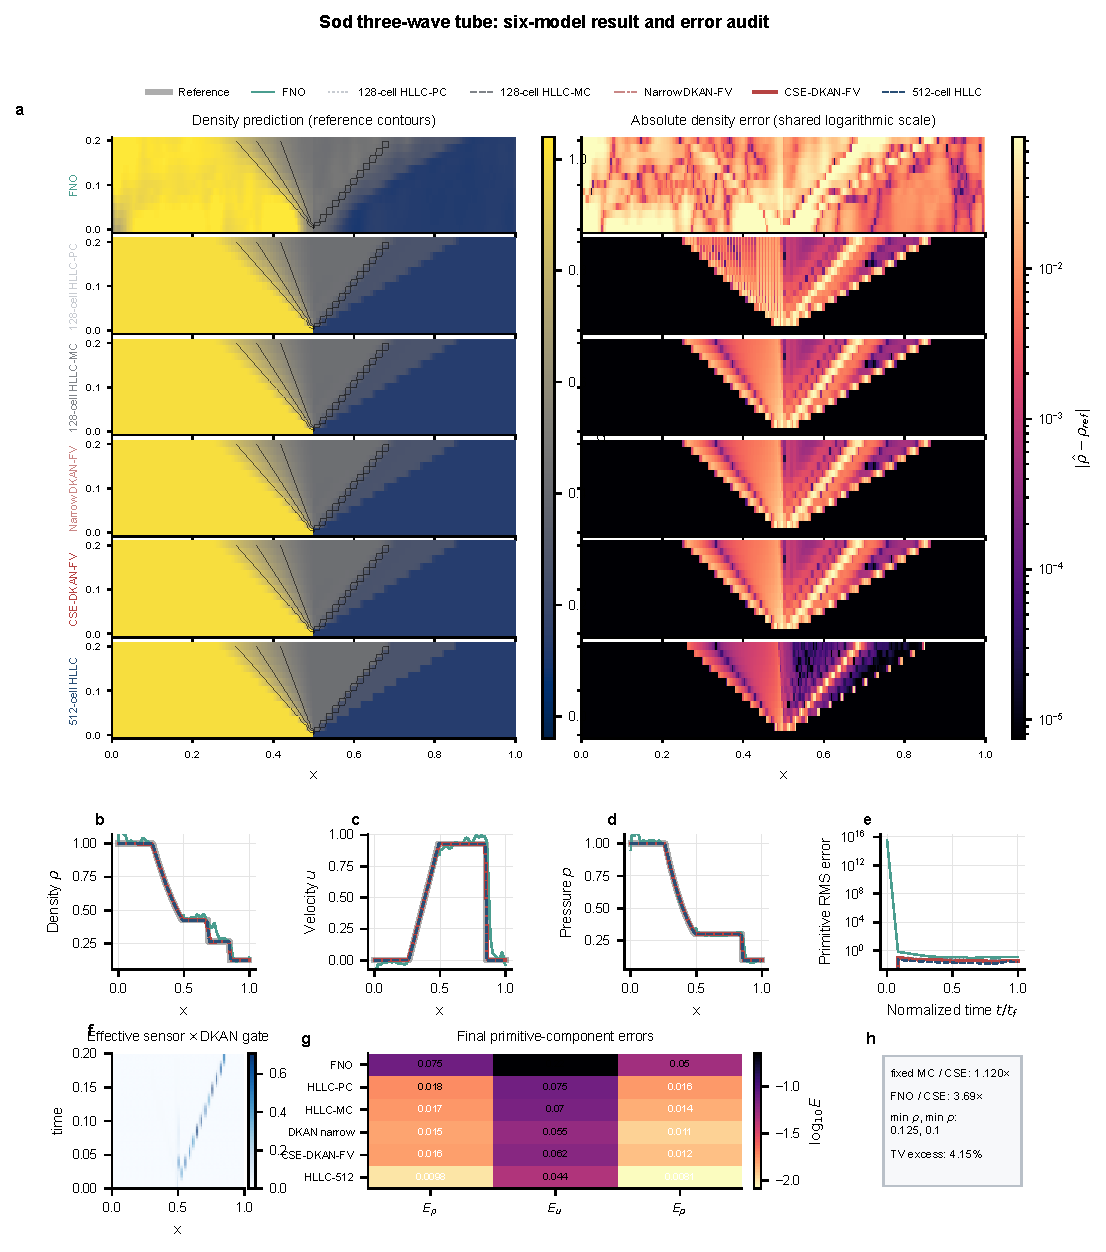
\includegraphics[width=0.82\textwidth]{fig13_mechanism_sod.pdf}
 \caption{Six-model Sod audit. \textbf{a}, For each model, density prediction with reference contours and co-registered absolute density error over $(x,t)$ on shared case-wise scales. \textbf{b--d}, Final density, velocity, and pressure. \textbf{e}, Time-resolved RMS evaluation loss. \textbf{f}, Effective sensor--DKAN gate. \textbf{g}, Final primitive-component errors. \textbf{h}, case summary. This layout is reused for Figs.~\ref{fig:mech_lax}--\ref{fig:mech_smooth}.}
 \label{fig:mech_sod}
\vspace{2pt}
\captionof{table}{Sod final-time error analysis. TV excess is relative to the reference density. Positivity columns report the minimum predicted density and pressure. Online time includes time integration for finite-volume rows and only the post-training forward pass for FNO.}
\label{tab:mech_sod}
\scriptsize\setlength{\tabcolsep}{4pt}
\begin{tabular}{lrrrrrrrr}
\toprule
Method & $E_\rho$ & $E_u$ & $E_p$ & $E_{\rm RMS}$ & TV$_\rho$ (\%) & $\min\rho$ & $\min p$ & Online (s)\\
\midrule
FNO & 0.07489 & 0.2242 & 0.05031 & 0.1390 & 92.42 & 0.1137 & 0.08289 & 0.00192\\
HLLC-PC & 0.01799 & 0.07451 & 0.01647 & 0.04527 & 2.103 & 0.1250 & 0.1000 & 0.6909\\
HLLC-MC & 0.01664 & 0.06977 & 0.01432 & 0.04223 & 2.103 & 0.1250 & 0.1000 & 0.6909\\
DKAN-FV narrow & 0.01536 & 0.05544 & 0.01109 & \textbf{0.03383} & 7.360 & 0.1250 & 0.1000 & 0.7117\\
\method{} & 0.01596 & 0.06207 & 0.01250 & 0.03770 & 4.145 & 0.1250 & 0.1000 & 0.7158\\
HLLC-512 & 0.009761 & 0.04444 & 0.008147 & 0.02669 & 1.319 & 0.1250 & 0.1000 & 3.292\\
\bottomrule
\end{tabular}
\end{figure*}

\subsubsection{Lax: stronger three-wave state transfer}

The Lax tube changes both pressure and velocity while retaining the three-wave topology. CSE lowers all three component errors and reduces RMS error from 0.07121 to 0.06320 (1.127-fold), the largest same-backbone gain among the two standard tubes. The improvement costs additional TV (2.73\% versus 0.719\%), but remains within the frozen trust envelope. The 512-cell result, 0.03573, quantifies the accuracy still available from actual grid refinement.

Unlike Sod, the Lax initial velocity is nonzero and the left-to-right pressure ratio is coupled to a mild density reversal. The resulting rarefaction, contact, and shock therefore occupy different characteristic speeds and state ranges from the dominant training archetype. The density error atlas shows that fixed MC and the narrow DKAN leave a broader contact/shock trace, whereas the engineering gate concentrates its correction on those paths. The component matrix confirms that the gain is not produced by trading one variable against another: density decreases by 7.4\%, velocity by 18.6\%, and pressure by 27.4\% relative to fixed MC.

At the earliest nonzero audit, CSE is marginally worse than fixed MC (0.09932 versus 0.09921), but it wins seven of twelve subsequent time points and ends 11.3\% lower. This crossing matters: the model does not simply reproduce a sharper initial step; its benefit appears after nonlinear wave separation. The narrow DKAN remains essentially identical to fixed MC despite its lower family validation loss, which rules out ``DKAN capacity alone'' as an explanation. FNO finishes at 0.2540 and the fine grid at 0.03573. Lax therefore provides the cleanest state-transfer result in the suite, but also shows that the learned correction is still a coarse-grid approximation rather than a substitute for resolution.

CSE requires 1.148~s online, only 2.0\% more than the shared 128-cell evolution, while 512-cell HLLC requires 5.020~s. The proposed/fine error ratio is nevertheless 1.77, so the relevant result is an intermediate accuracy--cost point. The TV increase is also localized rather than a global loss of admissibility: minimum density and pressure are unchanged from fixed MC, and the accepted reconstruction stays inside the declared 2\% candidate-to-fixed TV trust. Lax is therefore the strongest evidence that the gate can recognize a familiar wave topology in an unfamiliar state regime, rather than evidence that it supersedes a high-resolution shock-capturing method.

\begin{figure*}[p]
 \centering
 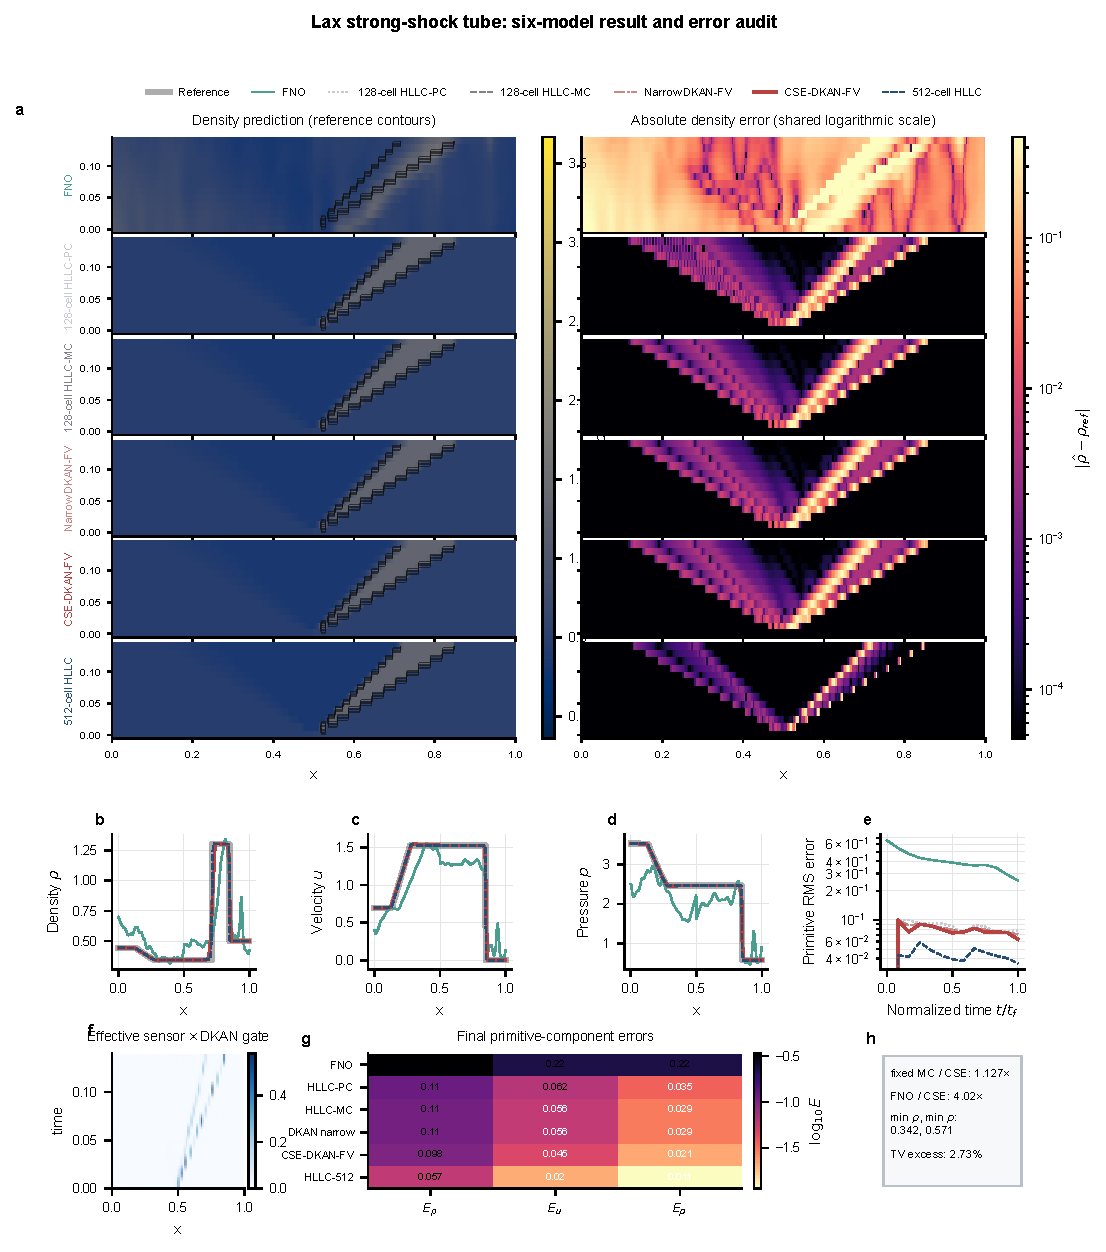
\includegraphics[width=0.82\textwidth]{fig14_mechanism_lax.pdf}
 \caption{Lax result and error audit. The learned correction reduces the rarefaction/contact/shock error bands and all three final component errors. Panel \textbf{e} shows that the advantage persists after wave separation; panel \textbf{f} localizes the effective gate to the discontinuity paths. Layout follows Fig.~\ref{fig:mech_sod}.}
 \label{fig:mech_lax}
\vspace{2pt}
\captionof{table}{Lax final-time error analysis; definitions follow Table~\ref{tab:mech_sod}.}\label{tab:mech_lax}
\scriptsize\setlength{\tabcolsep}{4pt}
\begin{tabular}{lrrrrrrrr}
\toprule Method & $E_\rho$ & $E_u$ & $E_p$ & $E_{\rm RMS}$ & TV$_\rho$ (\%) & $\min\rho$ & $\min p$ & Online (s)\\ \midrule
FNO & 0.3384 & 0.2205 & 0.2194 & 0.2540 & 96.95 & 0.3162 & 0.4652 & 0.00187\\
HLLC-PC & 0.1148 & 0.06245 & 0.03489 & 0.07808 & 0.706 & 0.3421 & 0.5710 & 1.125\\
HLLC-MC & 0.1061 & 0.05567 & 0.02909 & 0.07121 & 0.719 & 0.3421 & 0.5710 & 1.125\\
DKAN-FV narrow & 0.1062 & 0.05565 & 0.02907 & 0.07123 & 0.787 & 0.3421 & 0.5710 & 1.149\\
\method{} & 0.09833 & 0.04533 & 0.02111 & \textbf{0.06320} & 2.733 & 0.3421 & 0.5710 & 1.148\\
HLLC-512 & 0.05727 & 0.02050 & 0.01138 & 0.03573 & 0.736 & 0.3431 & 0.5710 & 5.020\\
\bottomrule\end{tabular}
\end{figure*}

\subsubsection{Moving contact: topology isolation}

This case removes shocks and rarefactions: velocity and pressure are constant, so only a moving density contact remains. The RMS score is consequently density-dominated. CSE changes 0.03767 to 0.03749, a 0.46\% gain, while the effective gate is nearly off (mean 0.000273; no final cell above 0.1) and adds no TV. The result is better interpreted as safe near-parity than as a material improvement. FNO's 1.066 error shows that the frozen global operator does not transfer to this unseen topology.

The isolated contact is diagnostically important because it removes the acoustic waves that can hide contact-specific behavior in Sod or Lax. Exact velocity and pressure remain constant, and all conservative finite-volume rows reproduce them to approximately $10^{-14}$. The nonzero error is therefore entirely due to density smearing. This is also why the legacy geometric-mean metric is invalid here: multiplying by two machine-zero component errors would make a visibly smeared contact appear almost exact. The preregistered RMS amendment preserves the physically active density contribution.

The contact error grows as the discontinuity crosses successive parent cells and peaks near $0.92t_f$. CSE is lower than fixed MC at seven of twelve audit times, but the differences are much smaller than the 128-to-512-grid gap. The final fine-grid density error is 0.03773, compared with 0.06494 for CSE. The near-zero effective gate indicates that the deterministic density threshold does not aggressively sharpen an already resolved contact. Consequently, this example supports topology-safe transfer and metric validity, not a strong accuracy claim. It also exposes the frozen FNO's lack of contact equivariance: its RMS error rises monotonically from 0.304 at the first audit to 1.066 at the final time.

The abstention is not automatic evidence that the contact branch is optimal. A lower density threshold might sharpen the front, but the v1 smooth-wave result shows the corresponding false-positive risk. The chosen 0.15--0.35 density ramp therefore encodes a precision--recall trade-off: strong isolated contacts are admitted, while small smooth density gradients are rejected. A future study should sweep contact amplitude and thickness under a frozen calibration set. In the present paper, retaining the fixed-MC error and zero TV excess is the defensible outcome because the contact case was not used to tune the threshold.

\begin{figure*}[p]
 \centering
 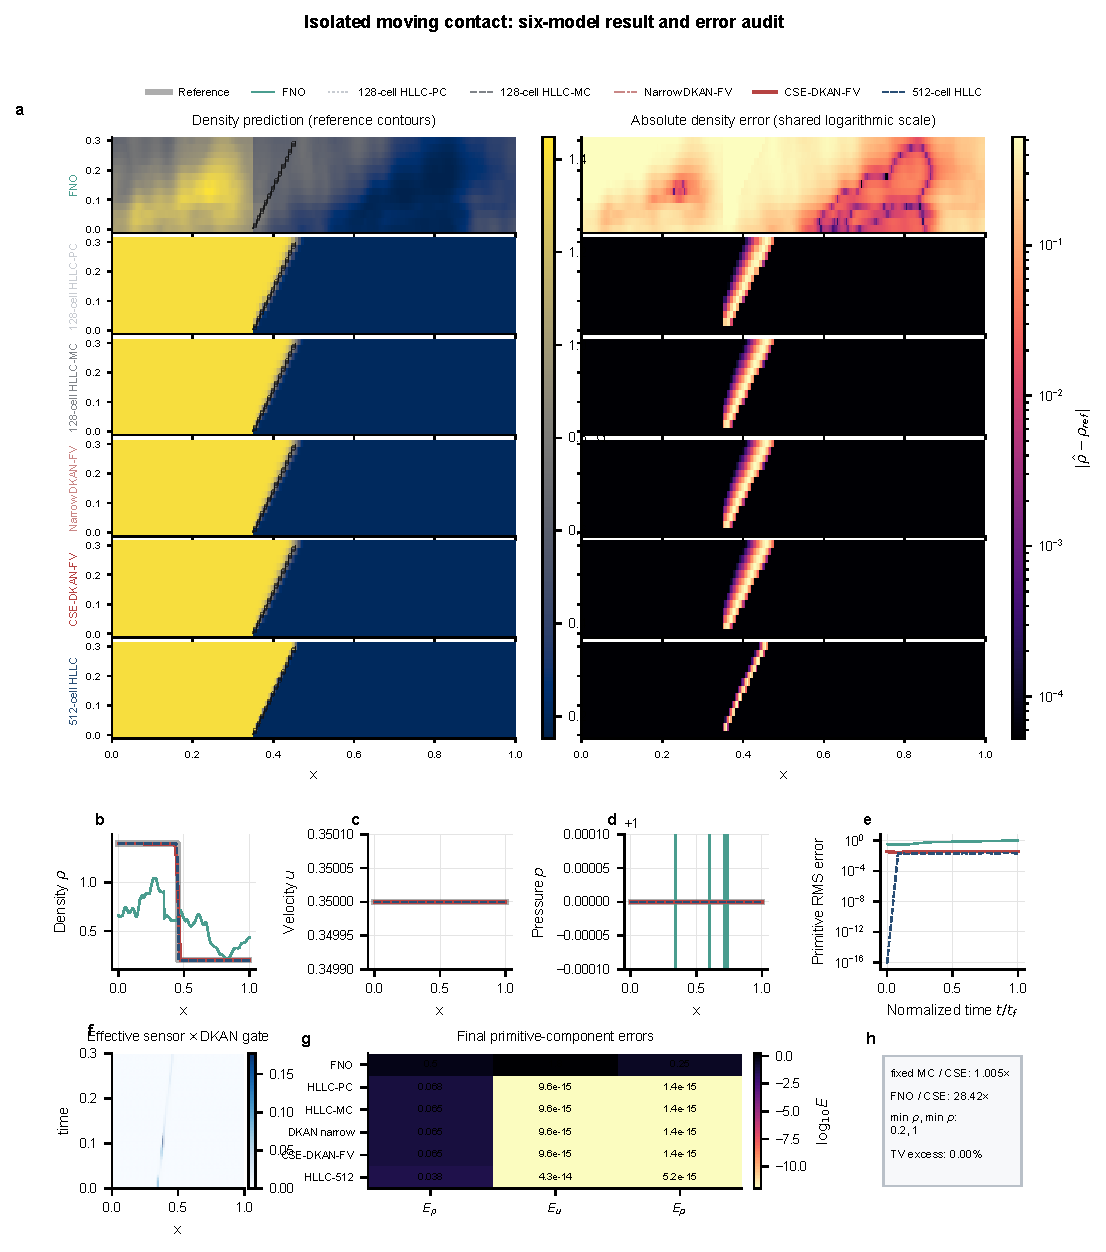
\includegraphics[width=0.82\textwidth]{fig15_mechanism_moving_contact.pdf}
 \caption{Moving-contact result and error audit. Velocity and pressure remain invariant, isolating density-contact resolution. The sensor suppresses most learned activity and CSE closely tracks fixed MC; the fine grid narrows the contact further. Layout follows Fig.~\ref{fig:mech_sod}.}
 \label{fig:mech_contact}
\vspace{2pt}
\captionof{table}{Moving-contact final-time error analysis; definitions follow Table~\ref{tab:mech_sod}.}\label{tab:mech_contact}
\scriptsize\setlength{\tabcolsep}{4pt}
\begin{tabular}{lrrrrrrrr}
\toprule Method & $E_\rho$ & $E_u$ & $E_p$ & $E_{\rm RMS}$ & TV$_\rho$ (\%) & $\min\rho$ & $\min p$ & Online (s)\\ \midrule
FNO & 0.5029 & 1.763 & 0.2494 & 1.066 & 108.1 & 0.2147 & 0.6775 & 0.00145\\
HLLC-PC & 0.06842 & $9.6\times10^{-15}$ & $1.4\times10^{-15}$ & 0.03950 & 0 & 0.2000 & 1.000 & 1.530\\
HLLC-MC & 0.06524 & $9.6\times10^{-15}$ & $1.4\times10^{-15}$ & 0.03767 & 0 & 0.2000 & 1.000 & 1.530\\
DKAN-FV narrow & 0.06524 & $9.6\times10^{-15}$ & $1.4\times10^{-15}$ & 0.03767 & 0 & 0.2000 & 1.000 & 1.550\\
\method{} & 0.06494 & $9.6\times10^{-15}$ & $1.4\times10^{-15}$ & \textbf{0.03749} & 0 & 0.2000 & 1.000 & 1.553\\
HLLC-512 & 0.03773 & $4.3\times10^{-14}$ & $5.2\times10^{-15}$ & 0.02178 & 0 & 0.2000 & 1.000 & 7.130\\
\bottomrule\end{tabular}
\end{figure*}

\subsubsection{Double rarefaction: expansion and positivity}

Two states moving apart form an expansion-dominated low-density centre. A shock-only model should abstain rather than sharpen it. CSE and fixed MC are statistically indistinguishable on the deterministic audit (0.016963 versus 0.016939; gain 0.9986), while density and pressure remain above 0.1152 and 0.03966. The maximum CSE/fixed TV ratio, 1.02053, occurs here and is consistent with the 2\% trust budget plus numerical tolerance. This controlled non-win is evidence of admissibility and selectivity, not of added resolution.

This problem tests a failure mode that cannot be represented by increasing shock strength in a standard tube. The two rarefaction fans move outward and create the smallest density and pressure in the suite. A discontinuity expert that confuses steep expansion gradients with compression can introduce an unphysical central kink or violate positivity. In the spatial panels, the four 128-cell conservative profiles remain smooth through the centre; CSE does not create a shock-like plateau. Its minimum state exactly matches the fixed-parent trajectory because the subcell positivity projection scales any inadmissible proposal toward MC.

The time-resolved score initially favors CSE (0.03112 versus 0.03154), but the curves cross and CSE wins only three of twelve nonzero audits. By $t_f$ the difference is 0.0000241 RMS, far too small to describe as an improvement. The effective gate has a mean of 0.01375, but only 1.56\% of final cells exceed 0.1; the TV projection caps the resulting variation. FNO reaches 1.085 and misses the low-density expansion, whereas 512-cell HLLC reaches 0.006505. The case documents positive states under an expansion-dominated shift and retains a marginal same-grid loss rather than omitting it.

The TV column illustrates why structural diagnostics require context. Fine HLLC has 3.17\% reference-relative density-TV excess, slightly larger than the coarse rows, even though its RMS error is much smaller. Here, additional resolution captures steeper fan edges rather than producing pathological oscillation. The trust constraint is accordingly defined relative to the fixed candidate path, not used as a surrogate objective for reference accuracy. For engineering use, the more important finding is that the constrained DKAN does not drive the rarefaction toward vacuum or create negative pressure when exposed to a mechanism absent from its supervised jump targets.

\begin{figure*}[p]
 \centering
 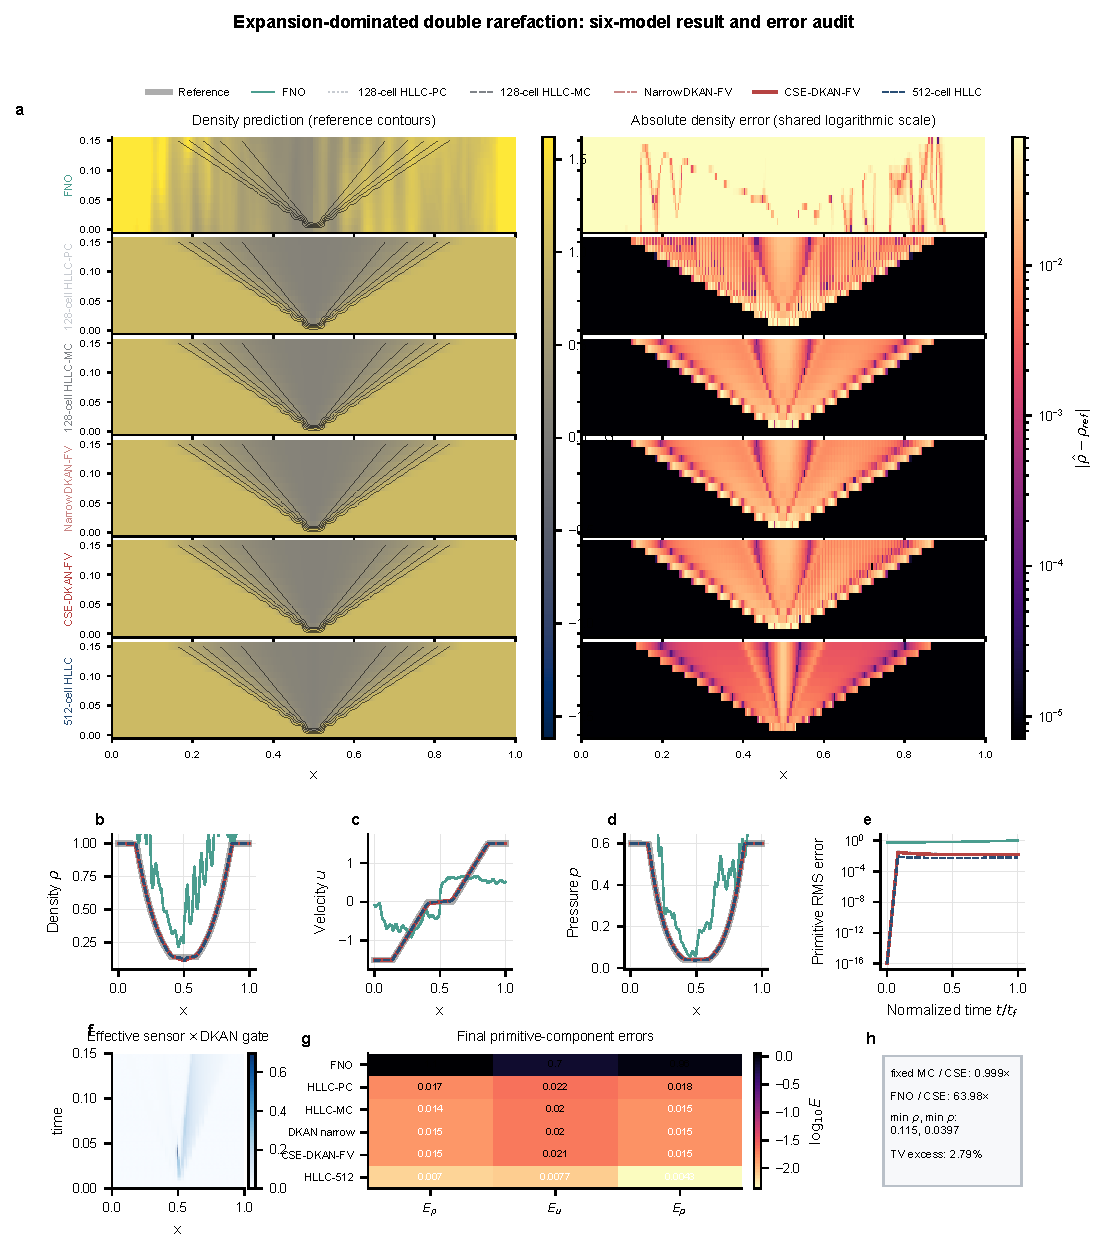
\includegraphics[width=0.82\textwidth]{fig16_mechanism_double_rarefaction.pdf}
 \caption{Double-rarefaction result and error audit. The central expansion remains positive and the learned path stays close to fixed MC. The FNO does not reproduce the expansion, while 512-cell HLLC gives the lowest RMS error. Layout follows Fig.~\ref{fig:mech_sod}.}
 \label{fig:mech_rarefaction}
\vspace{2pt}
\captionof{table}{Double-rarefaction final-time error analysis; definitions follow Table~\ref{tab:mech_sod}.}\label{tab:mech_rarefaction}
\scriptsize\setlength{\tabcolsep}{4pt}
\begin{tabular}{lrrrrrrrr}
\toprule Method & $E_\rho$ & $E_u$ & $E_p$ & $E_{\rm RMS}$ & TV$_\rho$ (\%) & $\min\rho$ & $\min p$ & Online (s)\\ \midrule
FNO & 1.145 & 0.7009 & 0.9585 & 1.085 & 679.2 & 0.2169 & 0.05567 & 0.00206\\
HLLC-PC & 0.01671 & 0.02230 & 0.01835 & 0.01926 & 2.612 & 0.1152 & 0.03966 & 0.8545\\
HLLC-MC & 0.01448 & 0.02048 & 0.01522 & \textbf{0.01694} & 2.612 & 0.1152 & 0.03966 & 0.8545\\
DKAN-FV narrow & 0.01450 & 0.02048 & 0.01525 & 0.01696 & 2.612 & 0.1152 & 0.03966 & 0.8722\\
\method{} & 0.01452 & 0.02050 & 0.01524 & 0.01696 & 2.786 & 0.1152 & 0.03966 & 0.8792\\
HLLC-512 & 0.007019 & 0.007705 & 0.004278 & 0.006505 & 3.171 & 0.1104 & 0.03736 & 3.692\\
\bottomrule\end{tabular}
\end{figure*}

\subsubsection{Colliding streams: compression topology}

Equal-pressure streams moving toward each other create a central compressed state bounded by two shocks, rather than a one-sided pressure-driven tube. CSE lowers every primitive error and improves RMS from 0.04415 to 0.04017 (1.099-fold). Its gate is localized (mean 0.00686; 1.56\% above 0.1), and TV excess is unchanged from fixed MC at 16.81\%. The symmetric benefit supports transfer of the local representation to a different interaction topology, although fine HLLC remains about twice as accurate.

Because the initial pressure and density are uniform, the wave system is driven entirely by converging momentum. This separates compression sensing from pressure-jump sensing: at early times the velocity indicator in Eq.~\eqref{eq:eulersensor} must activate before a strong pressure jump has formed. The resulting two-shock pattern is symmetric, so a biased correction would be visible as unequal front positions or an off-centre plateau. The CSE prediction preserves the symmetry and reduces density, velocity, and pressure errors by 8.7\%, 9.1\%, and 8.9\%, respectively.

The temporal audit shows an interaction-dependent benefit. Both coarse curves reach their largest error near $0.75t_f$, when the compressed region is most demanding; CSE is 0.04622 and fixed MC is 0.04792 there. CSE wins ten of twelve nonzero times and ends at 0.04017 versus 0.04415. Its TV excess equals that of fixed MC, so the improvement is not purchased through additional global oscillation. FNO's error grows to 0.4363, while the fine-grid value is 0.02197. Among the noncanonical cases, this is the clearest evidence that the learned correction responds to an unseen compression topology.

The added deployment cost is 0.0252~s over the shared 0.4480~s evolution, compared with 2.053~s for the 512-cell solve. Because all coarse reconstructions use identical parent means, the improvement comes from within-cell placement rather than a changed parent-grid trajectory. The result also clarifies the contact and rarefaction ties. The gate is not disabled everywhere outside Sod; it activates when local compression supplies a compatible signal.

\begin{figure*}[p]
 \centering
 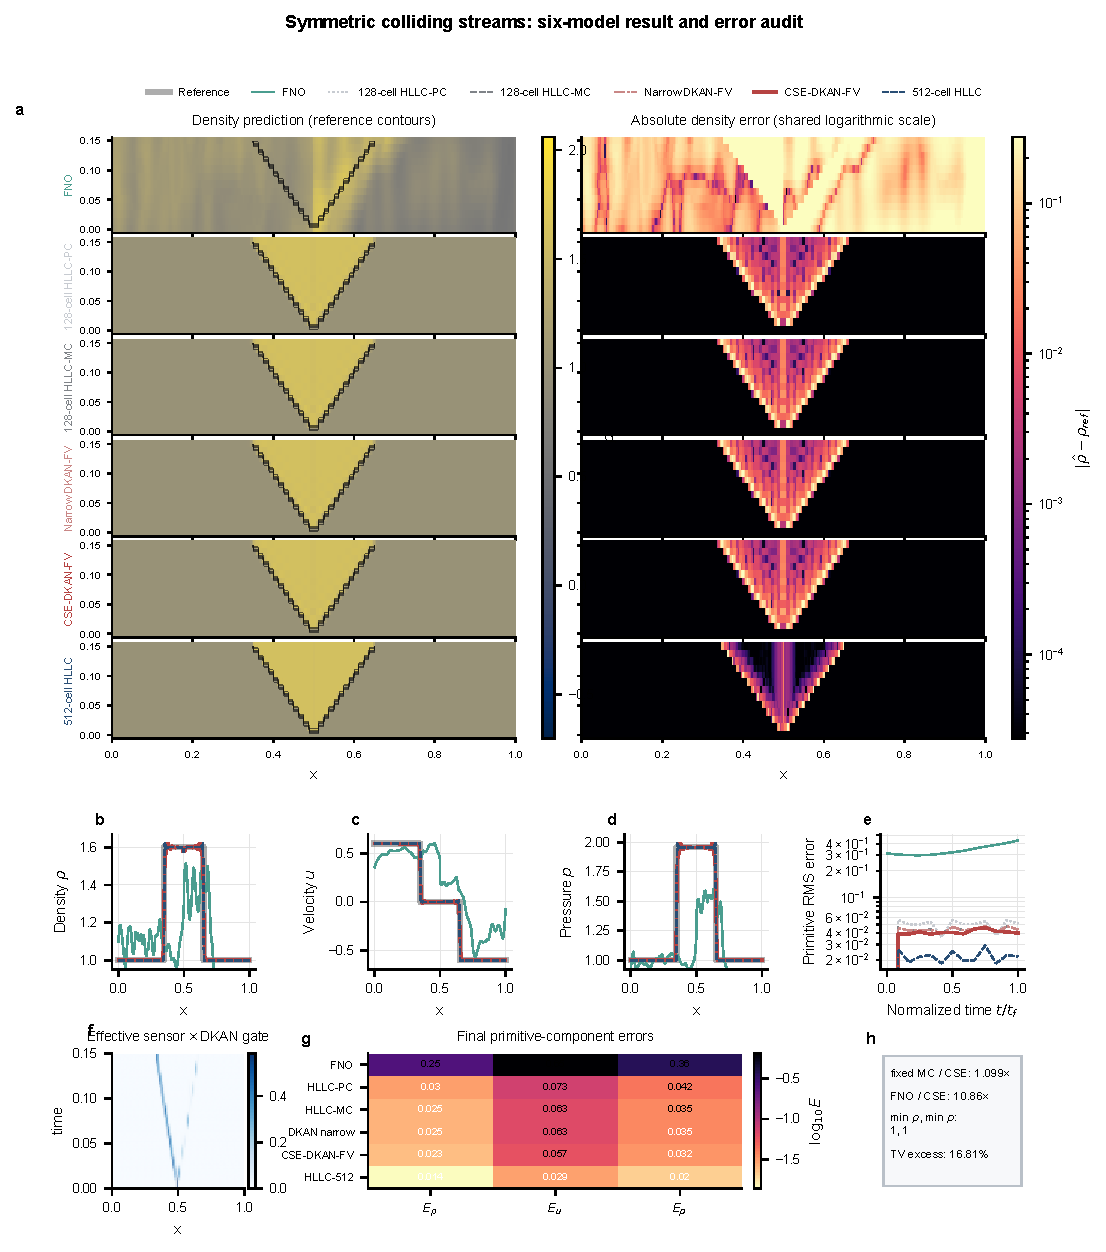
\includegraphics[width=0.82\textwidth]{fig17_mechanism_colliding_streams.pdf}
 \caption{Colliding-stream result and error audit. Two inward-moving compression fronts create a central high-density region. CSE reduces all final component errors with a localized gate, whereas FNO produces broad state errors. Layout follows Fig.~\ref{fig:mech_sod}.}
 \label{fig:mech_collision}
\vspace{2pt}
\captionof{table}{Colliding-stream final-time error analysis; definitions follow Table~\ref{tab:mech_sod}.}\label{tab:mech_collision}
\scriptsize\setlength{\tabcolsep}{4pt}
\begin{tabular}{lrrrrrrrr}
\toprule Method & $E_\rho$ & $E_u$ & $E_p$ & $E_{\rm RMS}$ & TV$_\rho$ (\%) & $\min\rho$ & $\min p$ & Online (s)\\ \midrule
FNO & 0.2452 & 0.6498 & 0.3573 & 0.4363 & 312.3 & 0.5936 & 0.4648 & 0.00189\\
HLLC-PC & 0.02950 & 0.07298 & 0.04165 & 0.05142 & 16.81 & 1.000 & 1.000 & 0.4480\\
HLLC-MC & 0.02507 & 0.06298 & 0.03538 & 0.04415 & 16.81 & 1.000 & 1.000 & 0.4480\\
DKAN-FV narrow & 0.02507 & 0.06297 & 0.03538 & 0.04414 & 16.81 & 1.000 & 1.000 & 0.4715\\
\method{} & 0.02288 & 0.05726 & 0.03224 & \textbf{0.04017} & 16.81 & 1.000 & 1.000 & 0.4732\\
HLLC-512 & 0.01365 & 0.02937 & 0.01999 & 0.02197 & 20.89 & 1.000 & 1.000 & 2.053\\
\bottomrule\end{tabular}
\end{figure*}

\subsubsection{Shu--Osher: shock--entropy-wave interaction}

The Shu--Osher problem confronts a shock with a high-frequency smooth density field absent from the Riemann training family \citep{shu1989eno2}. CSE (0.05765), fixed MC (0.05763), and narrow DKAN (0.05763) are effectively tied; the sensor is nearly off away from the shock (mean 0.00124; no final cell above 0.1). Thus, the method transports the unseen oscillatory structure without a measurable same-grid gain or extra TV. The 2048-versus-4096 reference disagreement is 0.00364 RMS, well below the coarse-model error but large enough to discourage interpreting the fourth decimal place.

This benchmark couples a discontinuity with a smooth spectrum, so neither universal sharpening nor universal smoothing is acceptable. The density atlas shows two spatially distinct requirements: localize the leading shock and retain the phase and amplitude of the downstream oscillations. All three 128-cell MC/DKAN profiles reproduce the large-scale phase, but their oscillation amplitudes remain more dissipative than the 512-cell result. The proposed sensor restricts the learned correction to the shock neighborhood; it does not treat every high-frequency density gradient as a contact.

CSE is below fixed MC at eight of twelve nonzero audit times, yet the ordering reverses at the final time by $2.56\times10^{-5}$ RMS. Their common error scale is about sixteen times the 2048--4096 reference disagreement and nearly three times the 512-cell error. These comparisons support stable mechanism transfer but not additional resolution of the entropy spectrum. FNO finishes at 0.7483 because the frozen Riemann-family operator misses both the upstream shocked state and the oscillatory tail. The result is therefore a useful negative boundary: local conservation and selective gating avoid catastrophic smoothing, but learning a Riemann jump blend alone does not recover the spectral benefit of additional grid points.

The cost increase from fixed MC to CSE is about 0.0203~s, whereas the 512-cell trajectory costs 8.124~s. A learned subcell model could therefore be attractive if its oscillation fidelity were improved, but the present checkpoint does not achieve that improvement. Phase-aware or gradient-spectrum losses, and training records containing smooth high-frequency structure, are plausible extensions. They are not retrofitted here because doing so after seeing Shu--Osher would convert a generalization test into a training case.

\begin{figure*}[p]
 \centering
 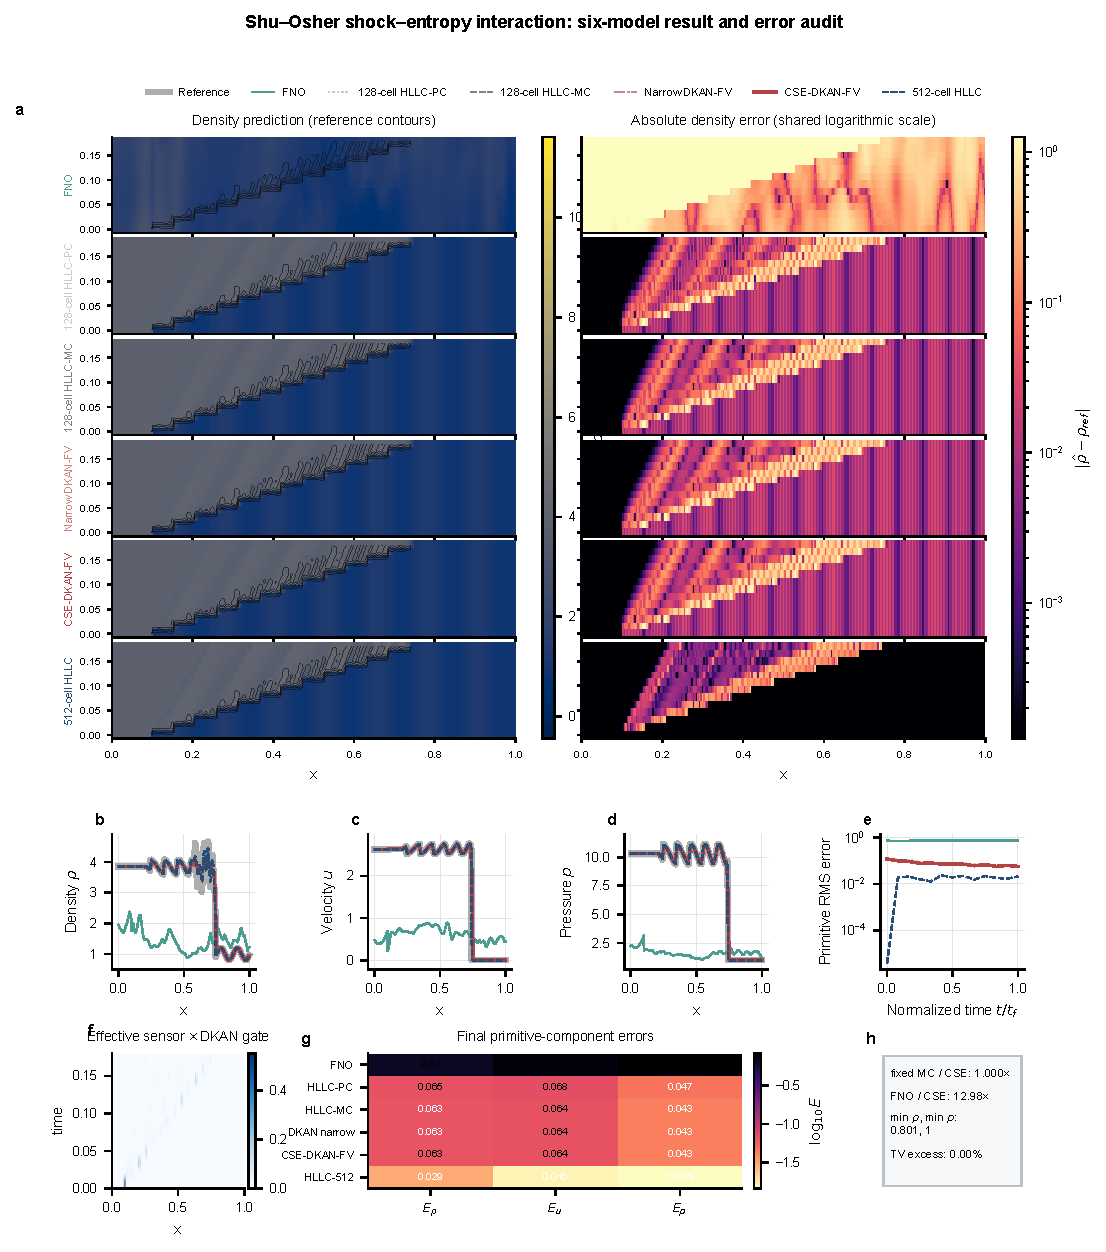
\includegraphics[width=0.82\textwidth]{fig18_mechanism_shu_osher.pdf}
 \caption{Shu--Osher result and error audit. The shock traverses an unseen smooth entropy wave. All conservative 128-cell reconstructions retain the oscillatory phase similarly; CSE is a near-tie with fixed MC, while FNO loses both the mean state and oscillations. Layout follows Fig.~\ref{fig:mech_sod}.}
 \label{fig:mech_shuosher}
\vspace{2pt}
\captionof{table}{Shu--Osher final-time error analysis; definitions follow Table~\ref{tab:mech_sod}.}\label{tab:mech_shuosher}
\scriptsize\setlength{\tabcolsep}{4pt}
\begin{tabular}{lrrrrrrrr}
\toprule Method & $E_\rho$ & $E_u$ & $E_p$ & $E_{\rm RMS}$ & TV$_\rho$ (\%) & $\min\rho$ & $\min p$ & Online (s)\\ \midrule
FNO & 0.6300 & 0.7560 & 0.8375 & 0.7483 & 0 & 0.7203 & 1.053 & 0.00188\\
HLLC-PC & 0.06459 & 0.06753 & 0.04679 & 0.06034 & 0 & 0.8005 & 1.000 & 2.142\\
HLLC-MC & 0.06306 & 0.06448 & 0.04276 & \textbf{0.05763} & 0 & 0.8005 & 1.000 & 2.142\\
DKAN-FV narrow & 0.06306 & 0.06448 & 0.04277 & 0.05763 & 0 & 0.8005 & 1.000 & 2.164\\
\method{} & 0.06311 & 0.06442 & 0.04285 & 0.05765 & 0 & 0.8005 & 1.000 & 2.163\\
HLLC-512 & 0.02935 & 0.01569 & 0.01433 & 0.02092 & 0 & 0.8000 & 1.000 & 8.124\\
\bottomrule\end{tabular}
\end{figure*}

\subsubsection{Woodward--Colella: interacting blast waves and walls}

The blast problem combines a $10^5$ pressure ratio, multiple discontinuities, reflecting boundaries, and wave collision \citep{woodward1984strongshocks}. CSE changes RMS from 0.23024 to 0.22887 (1.006-fold) and preserves positivity. This apparent 0.6\% same-grid gain is smaller than the 0.02424 RMS disagreement between 2048- and 4096-cell references, so it is reported as practical parity. The robust conclusion is weaker but useful: the Riemann-trained gate does not destabilize a multi-interface wall-bounded flow, and the fine-grid comparator still reduces error to 0.07761.

Woodward--Colella changes three assumptions simultaneously. It begins with two pressure discontinuities rather than one, the boundaries reflect rather than transmit waves, and the final state is created by repeated shock interaction rather than clean wave separation. The reconstruction gate has no explicit wall-distance feature. Nevertheless, its accepted correction remains sparse (mean 0.00887; 2.34\% of final cells above 0.1), preserves parent means to $5.68\times10^{-14}$, and does not approach the positivity floor. The FNO prediction reaches a pressure minimum of 0.00283, whereas all conservative coarse rows remain at 18.64 at the audited final state.

The error curves peak near $0.75t_f$, when the principal blast structures interact. CSE is then marginally worse than fixed MC (0.37279 versus 0.37225) and wins only four of twelve nonzero times; its small final advantage is therefore not temporally uniform. More importantly, the 2048--4096 reference disagreement is almost eighteen times the final CSE--fixed difference. The final protocol consequently uses 4096 cells and treats the two coarse reconstructions as tied. This conservative reading turns the case into a stability and boundary-transfer test, while the 512-cell error of 0.07761 shows that actual evolution-grid refinement remains the dominant accuracy mechanism for multi-shock interaction.

Runtime leads to the same conclusion. The DKAN output map adds only 0.0230~s to a 2.045~s coarse blast solve, whereas the 512-cell comparator requires 9.657~s; nevertheless, the finer evolution reduces RMS error by almost a factor of three. The case is therefore valuable precisely because it does not flatter the proposed model. It exposes the boundary of subcell-only learning: once error is dominated by coarse evolution through repeated interactions, redistributing conserved content inside the final parent cells has limited leverage.

\begin{figure*}[p]
 \centering
 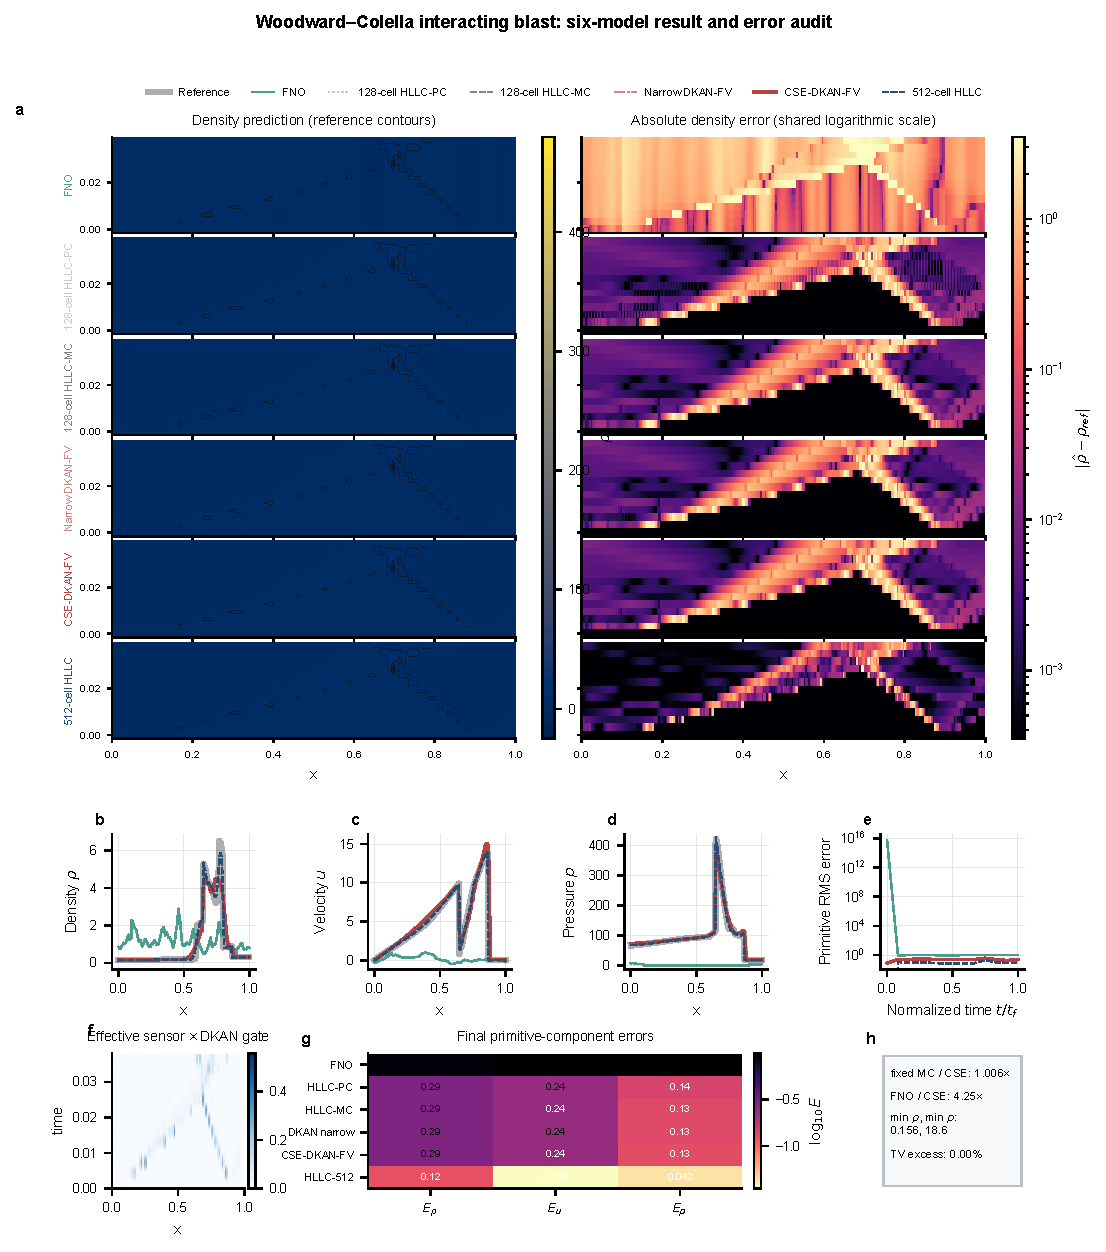
\includegraphics[width=0.82\textwidth]{fig19_mechanism_woodward_colella.pdf}
 \caption{Woodward--Colella interacting-blast result and error audit. The wave system includes wall reflection and repeated interaction. CSE remains positive and close to fixed MC, but the small apparent gain is below the independent reference-convergence floor. Layout follows Fig.~\ref{fig:mech_sod}.}
 \label{fig:mech_blast}
\vspace{2pt}
\captionof{table}{Woodward--Colella final-time error analysis against the 4096-cell reference; definitions follow Table~\ref{tab:mech_sod}.}\label{tab:mech_blast}
\scriptsize\setlength{\tabcolsep}{4pt}
\begin{tabular}{lrrrrrrrr}
\toprule Method & $E_\rho$ & $E_u$ & $E_p$ & $E_{\rm RMS}$ & TV$_\rho$ (\%) & $\min\rho$ & $\min p$ & Online (s)\\ \midrule
FNO & 0.9415 & 0.9895 & 0.9952 & 0.9732 & 24.27 & 0.2766 & 0.002835 & 0.00179\\
HLLC-PC & 0.2936 & 0.2416 & 0.1420 & 0.2343 & 0 & 0.1563 & 18.64 & 2.045\\
HLLC-MC & 0.2907 & 0.2396 & 0.1309 & 0.2302 & 0 & 0.1563 & 18.64 & 2.045\\
DKAN-FV narrow & 0.2907 & 0.2396 & 0.1308 & 0.2302 & 0 & 0.1563 & 18.64 & 2.067\\
\method{} & 0.2899 & 0.2386 & 0.1271 & \textbf{0.2289} & 0 & 0.1563 & 18.64 & 2.068\\
HLLC-512 & 0.1228 & 0.03481 & 0.04230 & 0.07761 & 0 & 0.1482 & 18.96 & 9.657\\
\bottomrule\end{tabular}
\end{figure*}

\subsubsection{Smooth entropy wave: specificity control}

The final case contains no discontinuity: an analytic periodic entropy wave is advected at constant velocity. It tests whether the learned correction perturbs a solution that requires no shock sharpening. With the sensor, CSE exactly matches fixed MC at $8.890\times10^{-5}$ RMS, its effective gate is zero, and TV excess is zero. The unsensed v1 model produced $3.430\times10^{-4}$, revealing false activation. This failure motivated the deterministic sensor, which was frozen before the v2/v3 reruns. The case therefore supports specificity rather than shock resolution.

The exact solution is a phase shift of the initial sinusoid, so amplitude damping, phase error, and spurious pressure or velocity coupling can be identified independently of a numerical Riemann reference. MC and sensor-gated CSE coincide at every one of the twelve nonzero audit times; the strict win counter is zero only because equality is not counted as a win. Their largest recorded RMS error is $1.954\times10^{-4}$ at the first audit and decreases to $8.890\times10^{-5}$. The 512-cell value is $7.734\times10^{-6}$, again showing the remaining truncation error.

The v1 failure is scientifically informative. A global TV budget alone permits a zero-mean learned redistribution that changes a smooth profile without increasing total variation beyond the allowed envelope. The explicit sensor supplies the missing local specificity and restores the fixed baseline exactly, with no network retraining or case-specific tuning. FNO peaks at 0.4898 near $0.75t_f$ and finishes at 0.4641; because this operator was not trained on the periodic family, the result measures transfer rather than best-achievable FNO accuracy. The negative control therefore validates the logic of the hybrid: learned sharpening must be conditional, and abstention is a successful outcome when the classical reconstruction is already appropriate.

This control also prevents the aggregate FNO/CSE gain from being overinterpreted. The 5220-fold ratio is dominated by a near-exact conservative baseline confronting an out-of-family operator, so the paper reports the minimum FNO/CSE gain (3.686) and the geometric aggregate (23.21) rather than an arithmetic mean. For the same reason, fixed/CSE equality is retained explicitly in the win count. These reporting choices keep the negative control informative without allowing it to manufacture a universal-superiority statistic.

\begin{figure*}[p]
 \centering
 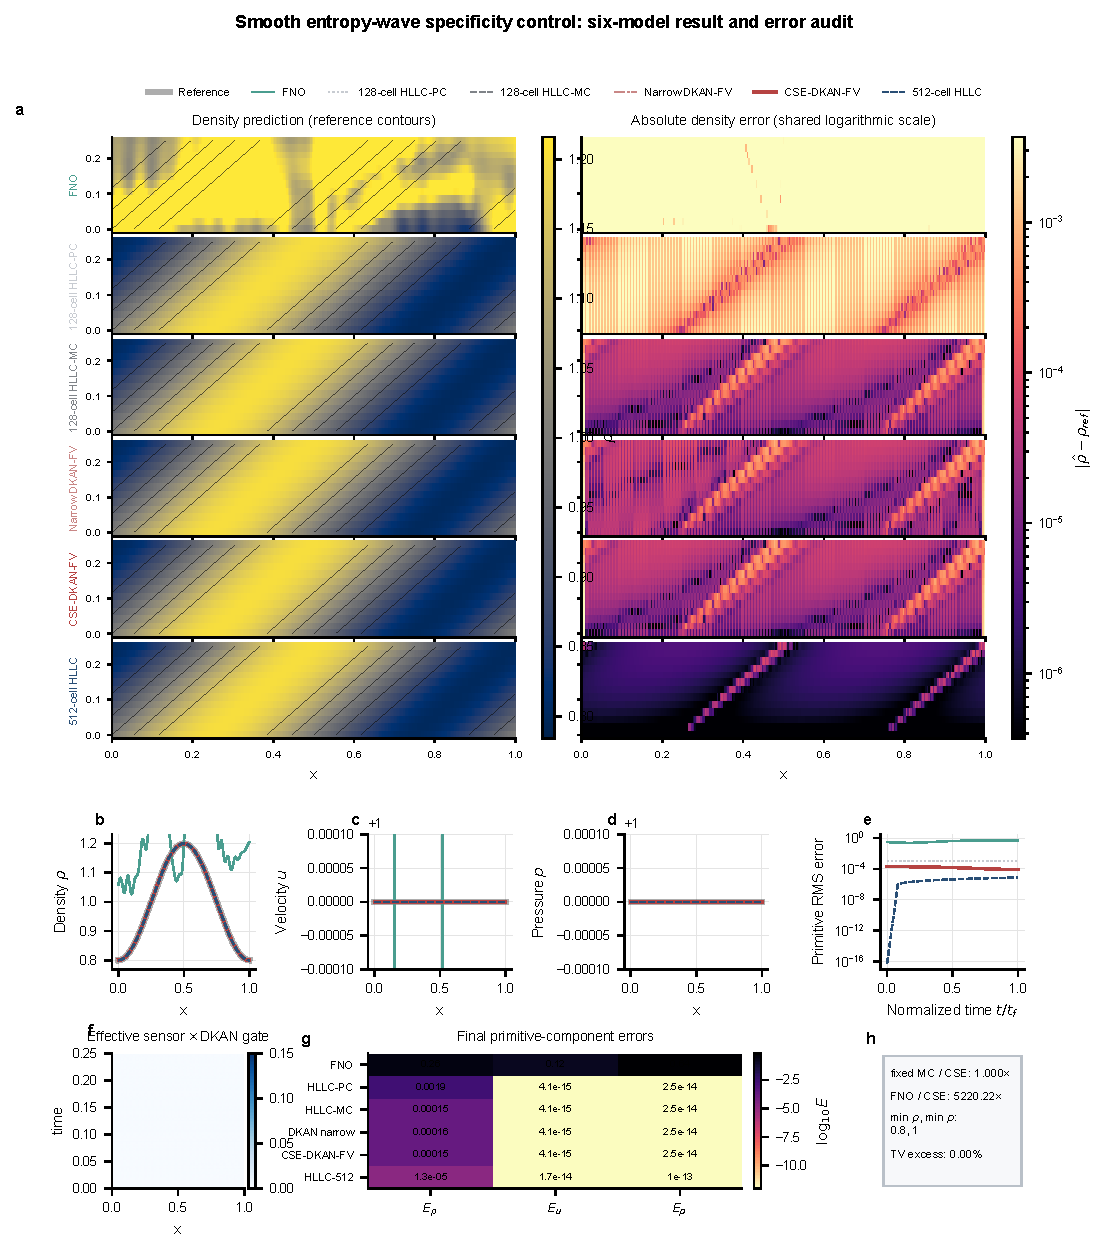
\includegraphics[width=0.82\textwidth]{fig20_mechanism_smooth_entropy.pdf}
 \caption{Smooth entropy-wave negative control. The sensor suppresses the learned correction, making CSE coincide with fixed MC and preserving the analytic phase and amplitude without added TV. FNO shows a large out-of-family amplitude and pressure error. Layout follows Fig.~\ref{fig:mech_sod}.}
 \label{fig:mech_smooth}
\vspace{2pt}
\captionof{table}{Smooth entropy-wave final-time error analysis; definitions follow Table~\ref{tab:mech_sod}.}\label{tab:mech_smooth}
\scriptsize\setlength{\tabcolsep}{4pt}
\begin{tabular}{lrrrrrrrr}
\toprule Method & $E_\rho$ & $E_u$ & $E_p$ & $E_{\rm RMS}$ & TV$_\rho$ (\%) & $\min\rho$ & $\min p$ & Online (s)\\ \midrule
FNO & 0.2565 & 0.1192 & 0.6442 & 0.4641 & 189.2 & 1.026 & 1.175 & 0.00251\\
HLLC-PC & 0.001927 & $4.1\times10^{-15}$ & $2.5\times10^{-14}$ & 0.001113 & 0 & 0.8005 & 1.000 & 0.9470\\
HLLC-MC & 0.0001540 & $4.1\times10^{-15}$ & $2.5\times10^{-14}$ & \textbf{$8.890\times10^{-5}$} & 0 & 0.8005 & 1.000 & 0.9470\\
DKAN-FV narrow & 0.0001556 & $4.1\times10^{-15}$ & $2.5\times10^{-14}$ & $8.986\times10^{-5}$ & 0 & 0.8005 & 1.000 & 0.9711\\
\method{} & 0.0001540 & $4.1\times10^{-15}$ & $2.5\times10^{-14}$ & $8.890\times10^{-5}$ & 0 & 0.8005 & 1.000 & 0.9716\\
HLLC-512 & $1.340\times10^{-5}$ & $1.7\times10^{-14}$ & $1.0\times10^{-13}$ & $7.734\times10^{-6}$ & 0 & 0.8001 & 1.000 & 4.291\\
\bottomrule\end{tabular}
\end{figure*}

\subsubsection{Sensor ablation and reference uncertainty}

Figure~\ref{fig:sensorablation} discloses the development sequence rather than presenting the sensor as a blind ablation. The v1 protocol was evaluated unchanged and exposed a smooth-wave regression. The deterministic sensor was then specified, thresholds were frozen, and all eight cases were rerun without retraining. It reduces smooth-wave error by 3.858-fold and Lax error by 5.75\%; it is neutral to within 0.6\% on five other cases and increases blast error by 2.9\%. Its value is therefore false-positive control, not a uniform accuracy boost.

\begin{figure*}[t]
 \centering
 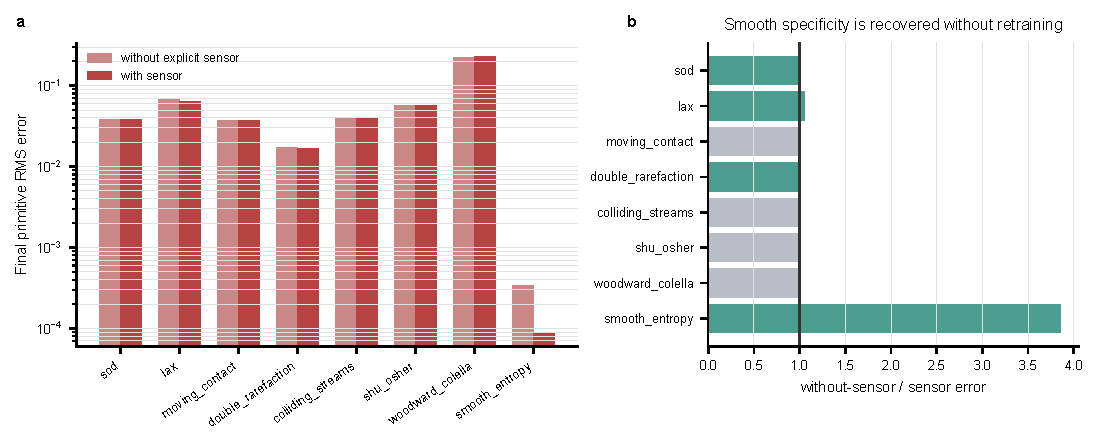
\includegraphics[width=0.90\textwidth]{fig21_sensor_ablation.pdf}
 \caption{Post-v1 deterministic sensor analysis. \textbf{a}, Final RMS error with and without Eq.~\eqref{eq:eulersensor}. \textbf{b}, Unsensed/sensed error ratio; values above one favor the sensor. The principal effect is recovery of the smooth negative control without neural retraining.}
 \label{fig:sensorablation}
\end{figure*}

The independent reference audit in Fig.~\ref{fig:referenceconvergence} compares 2048 and 4096 HLLC cells. Shu--Osher disagreement is 0.003639 RMS; Woodward--Colella disagreement is 0.02424. The latter triggered the only v3 reference amendment: the final blast reference was raised to 4096 cells while the cases, models, checkpoints, metrics, and comparator grids remained fixed. Maximum range-normalized pointwise disagreements are 0.0641 and 0.2040, respectively. These values are reported because a learned-versus-fixed difference below the reference floor cannot support a strong ranking.

\begin{figure*}[t]
 \centering
 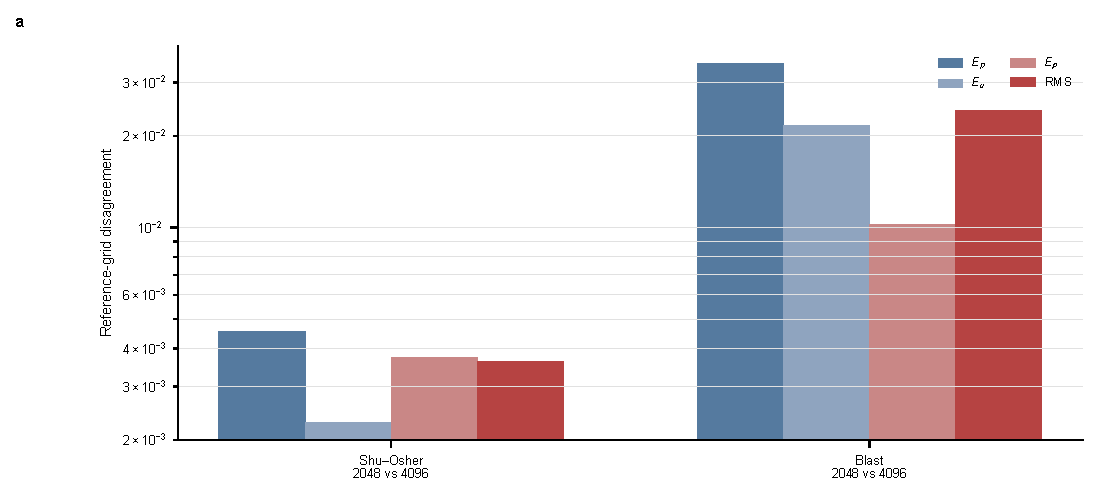
\includegraphics[width=0.72\textwidth]{fig22_reference_convergence.pdf}
 \caption{Reference-convergence audit for the two nonanalytic interaction cases. Bars show component and RMS disagreement between 2048- and 4096-cell HLLC solutions. The Woodward--Colella reference was consequently raised to 4096 cells in the final protocol.}
 \label{fig:referenceconvergence}
\end{figure*}

\FloatBarrier
\onecolumn
\noindent\begin{minipage}[t]{0.48\textwidth}
\small
\subsection{DKAN improves representation but does not impose conservation}
Table~\ref{tab:validation}\textbf{a} summarizes the five-seed canonical comparison. Direct DKAN-PINN lowered Burgers error from 0.2501 to 0.1602 and Sod error from 0.1731 to 0.08131 relative to MLP-PINN. The substitution therefore improved representation, especially for Euler, but did not impose hard conservation: its median Burgers mass drift was $7.76\times10^{-3}$, compared with $1.90\times10^{-3}$ for MLP-PINN.

\method{} reached 0.03117 on Burgers and 0.01863 on Sod. The fixed reconstructions reached 0.08761 and 0.01893. Thus, the same-backbone Euler increment was small on canonical Sod even though its reconstructed density shock was narrower. AV-PINN was the most accurate MLP-based PINN, while CI-PINN improved selected balance indicators at the expense of field error.
\end{minipage}\hfill
\begin{minipage}[t]{0.48\textwidth}
\small
\subsection{The predeclared cross-equation target is met}
The frozen v3 protocol passed every aggregate gate (Table~\ref{tab:validation}\textbf{b}). Burgers achieved a median gain of 1.8672 with a 95\% interval of [1.7828, 1.9392]; Euler achieved 1.0893 with [1.0864, 1.0913]. Their matched cross-equation gain was 1.4259 with [1.3952, 1.4523]. The lower bound exceeded 1.20, supporting the strong 20\% claim within the frozen one-dimensional scope.

All outputs preserved parent means within $4.44\times10^{-16}$; density and pressure remained positive, and no shock-entropy violation was detected. The maximum Rankine--Hugoniot residual ratio was 1.157, below its 1.20 gate. Twenty doubled-resolution WENO audits had a maximum normalized disagreement of $2.92\times10^{-4}$.
\end{minipage}

\vspace{5pt}
\begin{center}
\captionof{table}{Consolidated canonical and frozen validation. \textbf{a}, Canonical five-seed medians. Conservation is maximum Burgers mass drift and Euler energy-balance error, except for finite-volume rows, which report subcell mean preservation. \textbf{b}, Frozen v3 confirmation; intervals are bootstrapped over ten seed-level aggregates.}
\label{tab:validation}
\scriptsize
\textbf{a}\quad
\begin{tabularx}{0.94\textwidth}{Yrrrrrr}
\toprule
Method & $E_B$ & $w_B$ & $E_E$ & $w_E$ & Conserv. $B/E$ & Online $B/E$ (s)\\
\midrule
MLP-PINN & 0.2501 & 0.2009 & 0.1731 & 1.0000 & $1.90\times10^{-3}$/0.0919 & 0.00053/0.00043\\
GW-PINN & 0.2652 & 0.2225 & 0.1919 & 1.0000 & $2.19\times10^{-3}$/0.0505 & 0.00053/0.00040\\
AV-PINN & 0.1567 & 0.0607 & 0.1676 & 1.0000 & $1.61\times10^{-3}$/0.0869 & 0.00053/0.00043\\
CI-PINN & 0.2880 & 0.2610 & 0.2006 & 1.0000 & $1.01\times10^{-3}$/0.0242 & 0.00062/0.00049\\
DKAN-PINN & 0.1602 & 0.0660 & 0.08131 & 0.0851 & $7.76\times10^{-3}$/0.0113 & 0.00333/0.00211\\
Fixed MC + FV & 0.08761 & n/a & 0.01893 & n/a & 0/0 & 0.759/2.819\\
\method{} & \textbf{0.03117} & \textbf{0.00587} & \textbf{0.01863} & \textbf{0.00849} & $2.22\times10^{-16}$/$4.44\times10^{-16}$ & 0.762/2.852\\
\bottomrule
\end{tabularx}

\vspace{3pt}
\textbf{b}\quad
\begin{tabular}{lrrrrl}
\toprule
Branch & Seeds & Pairs & Median gain & Bootstrap 95\% CI & Decision\\
\midrule
Burgers amplitude--viscosity & 10 & 600 & 1.8672 & [1.7828, 1.9392] & pass\\
Euler Riemann--resolution & 10 & 300 & 1.0893 & [1.0864, 1.0913] & pass\\
Matched cross-equation & 10 & 10 aggregates & 1.4259 & [1.3952, 1.4523] & strong 20\% pass\\
\bottomrule
\end{tabular}

\vspace{4pt}
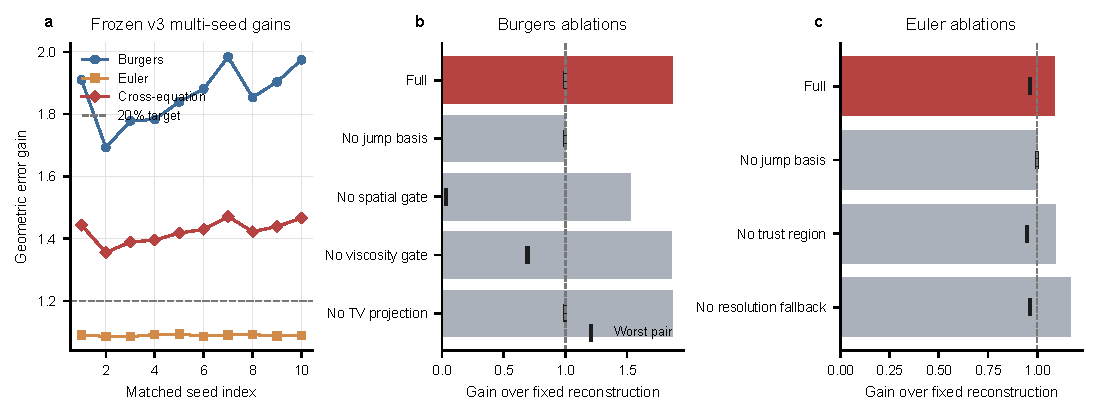
\includegraphics[width=0.78\textwidth]{fig11_multiseed_ablation.pdf}
\captionof{figure}{Seed stability and component analysis. \textbf{a}, Matched seed-level gains; the horizontal line marks the 1.20 target. \textbf{b,c}, Median ablation gain over fixed reconstruction; black ticks show the worst pair. Ablations are descriptive rather than an independent blind test.}
\label{fig:multiseed}
\end{center}
\clearpage
\subsection{The learned map occupies an intermediate accuracy--cost regime}

\begin{center}
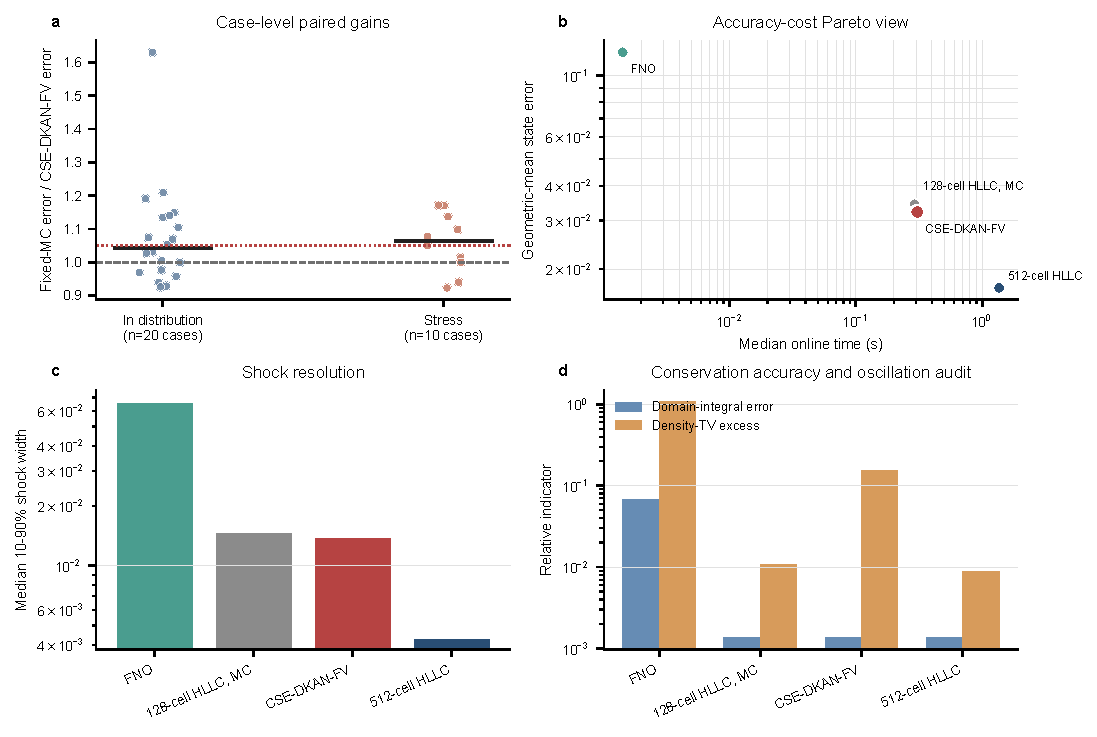
\includegraphics[width=0.70\textwidth]{fig10_engineering_benchmark.pdf}
\captionof{figure}{Engineering benchmark. \textbf{a}, Same-backbone gains. \textbf{b}, Online time versus error. \textbf{c}, Shock width. \textbf{d}, Domain-integral and density-TV indicators. FNO is fastest; 512-cell HLLC is most accurate.}
\label{fig:engineering}
\end{center}

\vspace{3pt}
\noindent\begin{minipage}[t]{0.58\textwidth}
\footnotesize
The 30-case Euler extension produced a Pareto result rather than universal dominance. On 20 in-distribution cases, \method{} had a geometric-mean state error of 0.03217. FNO reached 0.12125, giving a seed-level gain of 3.7687, but remained about 213 times faster online.

Against the same 128-cell HLLC backbone, fixed MC reached 0.03431. The paired median gain of \method{} was 1.0336, with a 95\% interval of [1.0102, 1.0747] and a 65\% win rate. The win-rate gate passed, but the preregistered 1.05 gain gate failed. On ten stress cases, the paired median gain was 1.0523 with a 66.7\% win rate.

The 512-cell HLLC method remained most accurate at 0.01713 but required 1.362~s. Hard reconstruction conservation was $1.78\times10^{-15}$ across all 30 cases and three seeds, and all finite-volume outputs retained positive density and pressure. The data therefore support a coarse conservative solver with a modest learned resolution gain, not a replacement for every fine-grid solve.

FNO had a median shock width of 0.06649, 6.77\% domain-integral error, and 106.8\% density-TV excess. CSE reached 0.01398, 0.136\%, and 15.4\%, respectively. Fixed MC and CSE had the same domain-integral error because they share evolved parent means; their difference is confined to subcell placement. Fine HLLC reduced width to 0.00435 and TV excess to 0.884\%, confirming that refinement remained the most reliable accuracy mechanism.

Cost comparisons represent different workflows. FNO performs one amortized forward pass; the finite-volume methods include time integration, and CSE adds reconstruction. FNO used 512 family-level training cases, whereas the engineering DKAN gate used 64 cases but many local stencil records. The reported timings therefore compare deployed implementations, not equal-data or equal-compute theoretical limits.
\end{minipage}\hfill
\begin{minipage}[t]{0.39\textwidth}
\centering
\captionof{table}{In-distribution engineering comparison. TV excess and domain error are relative to the exact solution; the TV-trusted row is post-registration.}
\label{tab:engineering}
\scriptsize
\resizebox{\linewidth}{!}{%
\begin{tabular}{lrrrrr}
\toprule
Method & State error & Online (s) & Shock width & TV excess & Domain error\\
\midrule
FNO & 0.12125 & 0.00143 & 0.06649 & 106.8\% & 6.77\%\\
128-cell HLLC + fixed MC & 0.03431 & 0.2918 & 0.01476 & 1.08\% & 0.136\%\\
128-cell \method{} & 0.03217 & 0.3057 & 0.01398 & 15.4\% & 0.136\%\\
128-cell \method{}, 2\% TV trust & 0.03300 & $\approx$0.306 & 0.01431 & 3.10\% & 0.136\%\\
512-cell HLLC & \textbf{0.01713} & 1.362 & \textbf{0.00435} & 0.884\% & 0.136\%\\
\bottomrule
\end{tabular}}

\vspace{8pt}
\raggedright
\footnotesize
\subsection{TV control removes unsafe corrections at modest accuracy cost}
\label{sec:tvtrust}

The unprojected model reduced state error but increased median density-TV excess to 15.5\%. A 2\% budget accepted a median DKAN multiplier of 0.567, reduced exact-reference TV excess to 3.10\%, retained a paired gain of 1.0348, and raised the win rate to 70\%. Larger budgets reduced state error slightly but increased TV monotonically.

Near-constant stress cases make geometric means artificially small, so paired gains and case distributions are also reported. Because the TV study was designed after the main benchmark, it is diagnostic rather than independent confirmation.
\end{minipage}
\clearpage
\noindent\begin{minipage}[t]{0.44\textwidth}
\footnotesize
\subsection{The learned basis drives accuracy while rejection controls tails}

The ablations assign different roles to accuracy and risk control. Removing the Burgers jump basis eliminates the median gain, identifying the explicit discontinuity profile as the source of sharpening. The remaining interventions change typical error much less than the worst case. Without the spatial or viscous-width gate, the worst-pair gain falls to 0.0356 or 0.6934. The TV projection reduces maximum TV excess from 4.25\% to 3.13\% without changing the median gain. For Euler, removing the trust factor or resolution fallback can improve the median while raising the maximum Rankine--Hugoniot ratio to 1.209 or 1.616. Mean error alone would therefore select riskier variants.

The diversified suite adds a specificity ablation that the original Riemann-only study could not expose. Without the explicit sensor, the smooth entropy-wave error is $3.430\times10^{-4}$, 3.86 times the sensor-enabled value, even though the correction remains conservative. Equation~\eqref{eq:eulersensor} restores exact parity with fixed MC without retraining. Its effect on shock cases is deliberately smaller: Lax improves by 5.75\%, Sod by 0.078\%, and the blast case regresses by 2.9\%. The sensor should therefore be interpreted as a rejection policy rather than an independent source of accuracy.

Primitive-component errors distinguish genuine gains from benign abstention. On Lax, CSE reduces $(E_\rho,E_u,E_p)$ from $(0.1061,0.05567,0.02909)$ to $(0.09833,0.04533,0.02111)$. On colliding streams it reduces all three components by about 8.8--9.1\%. Conversely, double rarefaction, Shu--Osher, and the smooth negative control remain at fixed-MC accuracy. The learned basis therefore recovers part, but not all, of the benefit supplied by additional parent cells; it is not consistently better than a fixed limiter when the required mechanism is expansion or smooth transport.

\section{Engineering application hypotheses}

The validated equation class is limited to one-dimensional scalar and ideal-gas Euler conservation laws. Table~\ref{tab:applications} therefore ranks migration directions rather than claiming deployment. The closest candidates preserve Riemann-wave structure and conservative cell averages; each still requires domain-specific equations, source terms, boundary conditions, and validation data.

Gas pipelines and quasi-one-dimensional ducts are the most direct Euler extensions. Traffic flow is the closest scalar application and has motivated conservative neural finite-volume research \citep{lichtle2025unfv}. Hydraulic and multiphase systems add wet/dry states, complex equations of state, or nonconservative products, and therefore require new admissible sets rather than simple retraining.
\end{minipage}\hfill
\begin{minipage}[t]{0.53\textwidth}
\centering
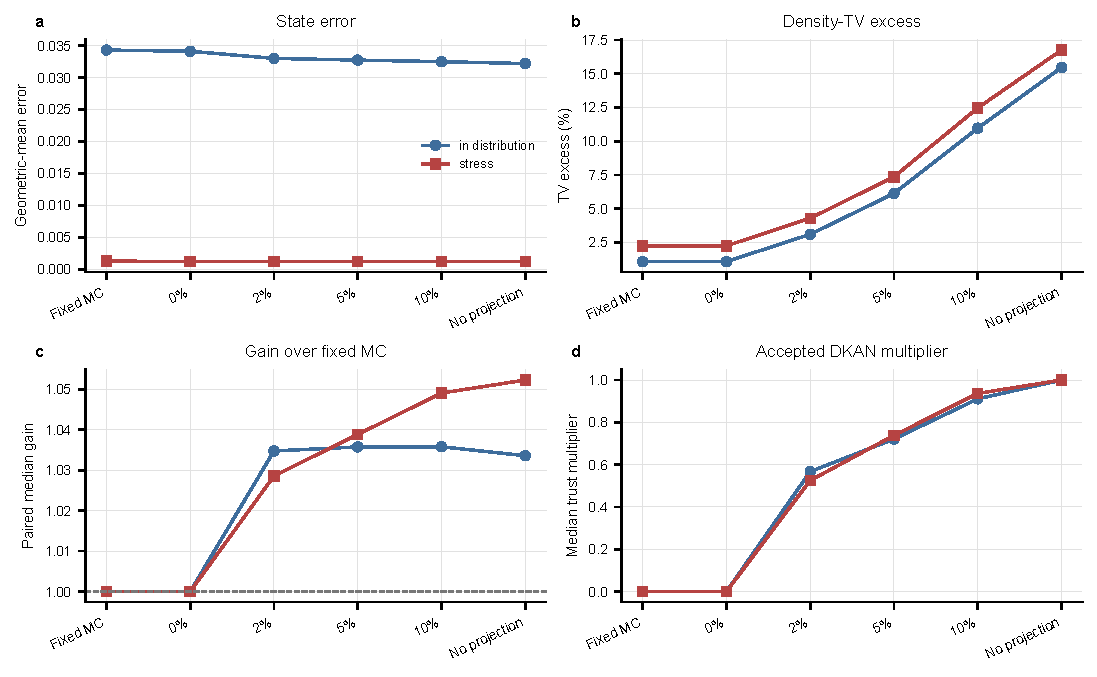
\includegraphics[width=\linewidth]{fig12_tv_trust_diagnostic.pdf}
\captionof{figure}{Post-registration density-TV trust study. \textbf{a}, Geometric-mean state error. \textbf{b}, Median density-TV excess. \textbf{c}, Paired gain over fixed MC. \textbf{d}, Accepted global DKAN multiplier. A 2\% budget provides most of the accuracy gain while rejecting nearly half of the unprojected correction.}
\label{fig:tvtrust}

\vspace{5pt}
\captionof{table}{Descriptive ablation summary on the frozen v3 cases. Worst-pair gain below one indicates a case where the variant is less accurate than fixed MC.}
\label{tab:ablation}
\scriptsize
\resizebox{\linewidth}{!}{%
\begin{tabular}{llrrr}
\toprule
Equation & Variant & Median gain & Worst-pair gain & Safety indicator\\
\midrule
Burgers & Full model & 1.8672 & 1.0000 & max TV excess 3.13\%\\
Burgers & No jump basis & 1.0000 & 1.0000 & max error $4.44\times$ full\\
Burgers & No spatial jump gate & 1.5302 & 0.0356 & max TV excess 4.82\%\\
Burgers & No viscous-width gate & 1.8625 & 0.6934 & max error $1.44\times$ full\\
Burgers & No TV projection & 1.8672 & 1.0000 & max TV excess 4.25\%\\
\midrule
Euler & Full model & 1.0893 & 0.9647 & max RH ratio 1.157\\
Euler & No jump basis & 1.0000 & 1.0000 & max RH ratio 1.000\\
Euler & No trust factor & 1.0929 & 0.9482 & max RH ratio 1.209\\
Euler & No resolution fallback & 1.1716 & 0.9637 & max RH ratio 1.616\\
\bottomrule
\end{tabular}}

\vspace{9pt}
\captionof{table}{Candidate engineering directions. Evidence level refers to proximity to the present equations, not to completed application validation.}
\label{tab:applications}
\scriptsize
\renewcommand{\arraystretch}{1.0}
\begin{tabularx}{\linewidth}{P{0.28\linewidth}Y}
\toprule
Direction & Migration hypothesis and required validation\\
\midrule
Gas-pipeline pressure waves & High structural match. Use DKAN subcells to localize compression fronts. Validate friction, a real-gas equation of state, junction conservation, and field sensors.\\
Quasi-1D ducts and inlet unstart & High shock/contact match. Reconstruct fronts in operating-envelope sweeps. Validate area and source terms, moving boundaries, and multidimensional separation.\\
Water hammer and dam-break waves & Moderate-to-high match. Reconstruct hydraulic jumps and steep pressure fronts. Validate the pipe or shallow-water model, wet/dry positivity, and cavitation.\\
Traffic kinematic waves & High scalar-law match. Reconstruct stop-and-go and queue fronts. Validate nonconvex fluxes, network nodes, and heterogeneous trajectory data.\\
Reactive or multiphase shock tubes & Moderate match. Extend the jump basis to species and phases. Validate stiff chemistry, phase admissibility, and new entropy and positivity constraints.\\
\bottomrule
\end{tabularx}
\end{minipage}
\twocolumn

\section{Discussion}

The results support the central restriction placed on learning. Direct DKAN-PINN improved canonical shock representation but retained measurable mass drift. In contrast, the subcell model preserved parent means to floating-point precision because every correction satisfies Eq.~\eqref{eq:nullspace}. Conservation therefore follows from the admissible function space, not from successful optimization. The comparison does not prove that the null-space restriction alone lowers field error, but it isolates conservation from approximation quality.

The strongest accuracy claim remains the preregistered cross-equation statistic. Its 1.4259 gain exceeded the 1.20 threshold, although the contribution was uneven across equations. Burgers reached a 1.8672 median gain, whereas Euler reached 1.0893. The broader engineering benchmark also missed its predeclared 1.05 same-grid gain threshold. Reporting the cross-equation result without these branch and deployment results would overstate generality.

The mechanism suite explains where the learned map transfers. Its clearest benefits occur for Lax and colliding-stream compression. Contacts, expansion, Shu--Osher oscillations, and smooth advection remain near fixed-MC accuracy. The blast ranking is unresolved because reference disagreement exceeds the learned-versus-fixed difference. This pattern is consistent with selective compression-aware transfer, not a generally superior edge architecture. The narrow DKAN's low validation loss but weaker rollout performance further shows that calibration distribution matters.

A posteriori rejection affects risk more than median accuracy. The viscous-width gate, trust factor, and resolution fallback changed typical errors little, but prevented large worst-pair or Rankine--Hugoniot regressions. This asymmetry makes mean error an insufficient model-selection criterion. It also explains why the smooth negative control is part of the evidence rather than an illustrative extra.

The comparators occupy distinct deployment regimes. FNO provides millisecond inference after substantial offline data generation and training, but transferred poorly outside its training family here. Fine-grid HLLC gives the lowest error and narrowest shocks at the largest online cost. \method{} lies between them: it preserves a coarse conservative trajectory and recovers a modest part of the refinement benefit. The preferable regime depends on the required balance among latency, accuracy, and invariant preservation.

The evidence has six important boundaries. The subcell network is supervised by WENO or exact Riemann data and is not data-free. Its reference and training costs require repeated deployment to amortize. The deterministic sensor was designed after the disclosed v1 smooth-wave failure, although its thresholds were frozen before v2/v3 evaluation. Entropy is audited rather than imposed as a hard constraint. All tests remain one-dimensional and use an ideal-gas Euler model. The global density-TV projection does not yet provide a face-consistent multidimensional policy. Finally, the frozen FNO comparison is not an equal-data, retrained operator study.

\section{Conclusion}

This study tested whether neural shock reconstruction becomes more reliable when learning is confined to zero-mean subcell structure. Within one-dimensional Burgers and Euler problems, the restriction preserved the conservative parent trajectory independently of training and exceeded the predeclared cross-equation accuracy threshold. Direct DKAN-PINN improved representation but did not obtain the same conservation property.

The broader evidence defines a narrower practical claim. Same-grid engineering improvement was 3.36\%, and the mechanism suite achieved a 1.0429 geometric gain with five wins. Fine-grid HLLC remained more accurate, while FNO remained much faster. \method{} should therefore be viewed as a selective coarse-grid reconstruction strategy, with its clearest advantage on localized compression fronts. Multidimensional tests and application-specific admissibility sets are required before engineering deployment.

\appendix

\section{Implementation and reproducibility ledger}

The study separates four experiment roles. Canonical single-problem PINNs test whether changing the field approximator from MLP to DKAN improves shock representation. The original frozen v3 suite tests the preregistered cross-equation claim with ten matched seeds and no post-freeze checkpoint selection. The 30-case engineering suite tests family-level deployment with three FNO and three DKAN-FV seeds. Finally, the mechanism-diverse v1--v3 suite reuses those frozen checkpoints on eight physically distinct Euler cases. Mixing these roles would inflate the apparent sample size and obscure which evidence supports which claim.

Table~\ref{tab:implementation} records the settings that determine the learned comparators. The canonical MLP-PINN, GW-PINN, AV-PINN, and CI-PINN use the same MLP within each equation. Direct DKAN-PINN uses a near-matched parameter budget. The narrow and engineering DKAN-FV models share the same 15--16--1 edge-function architecture but differ in their training distributions. Only the blend network is optimized; the HLLC update, MC basis, jump basis, and projections are fixed algorithms. The FNO is trained on complete 512-point fields and therefore uses more family-level cases and parameters than the local DKAN gate.

\begin{table*}[t]
\centering
\caption{Training and evaluation ledger. ``B/E'' denotes Burgers/Euler. DKAN-FV has 3089 trainable gate parameters within a 6284-parameter implementation that also records fixed reconstruction logic.}
\label{tab:implementation}
\scriptsize
\begin{tabularx}{\textwidth}{P{0.18\textwidth}P{0.16\textwidth}P{0.18\textwidth}P{0.12\textwidth}P{0.13\textwidth}Y}
\toprule
Model family & Seeds and precision & Training data & Iterations / batch & Parameters & Optimization and evaluation role\\
\midrule
Canonical MLP PINNs & 5; float64 & One canonical problem per equation; fresh collocation batches & 1000/512 (B); 800/256 (E) & 8641/8707 & Strong, gradient-weighted, artificial-viscosity, or coupled integral objective; descriptive comparison\\
Direct DKAN-PINN & 5; float64 & Same canonical problems and batch counts & 1000 (B); 800 (E) & 8562/8475 & Replaces the MLP field network while retaining pointwise residual training\\
Narrow DKAN-FV & 10 trained; 3 used in case plates; float64 & 20 Sod-neighbourhood cases; 100/200/400 cells; 8 subcells; $t=0.2$ & 2500/1024 & 3089 trainable; 6284 total & Distribution-shift comparator; frozen checkpoints reused without tuning\\
Engineering \method{} & 3; float64 & 64 Riemann cases; 64/128 cells; 4 subcells; $t\in\{0.08,0.16,0.28\}$ & 2500/1024 & 3089 trainable; 6284 total & Adam, $10^{-3}$; gradient norm clipped at 10; family-level gate\\
FNO & 3; float32 & 512 training and 128 validation cases; 512 points & 2000/8 & 105027 & AdamW, $2\times10^{-3}$, cosine decay to $5\times10^{-5}$, weight decay $10^{-5}$\\
HLLC-PC/MC/512 & deterministic; float64 & No learned data & not applicable & 0 & Numerical baselines and fine-grid accuracy reference\\
\bottomrule
\end{tabularx}
\end{table*}

Within each Euler case, the 128-cell PC, MC, narrow DKAN, and engineering DKAN rows share the same evolved parent-cell averages, HLLC flux, SSP-RK3 update, and case-specific boundary condition. Their final differences therefore arise only from the observation or reconstruction map. Outflow is used for the Riemann, contact, rarefaction, collision, and Shu--Osher cases; the blast uses reflecting walls and the smooth control is periodic. The 512-cell HLLC baseline instead changes the evolution grid and is interpreted as an accuracy--cost reference. FNO predicts the complete field directly and does not share the finite-volume trajectory.

Timing comparisons are deployment measurements rather than hardware-independent complexity results. FNO timing is a post-training forward pass; finite-volume timing includes time integration, and DKAN-FV timing adds reconstruction. Offline reference generation and optimization are reported separately where available. \todoauthor{Before submission, record the exact CPU, GPU, driver, PyTorch build, thread count, warm-up protocol, and number of timing repeats used for the final timing table.}

\section{Diagnostic interpretation and failure taxonomy}

The detailed case plates prevent three common overinterpretations. First, a low family-level validation loss does not guarantee held-out rollout accuracy: the narrow DKAN has the lowest internal loss but does not dominate the diversified suite. Second, a nonzero learned correction is not always beneficial; expansion, smooth transport, and high-frequency entropy waves require abstention or near-parity. Third, algebraic conservation does not guarantee a nonoscillatory profile. Every CSE reconstruction preserves its parent means, yet a misplaced local blend can still increase TV. The smooth-wave v1 failure is the clearest example: conservation held while accuracy regressed.

\begin{table*}[t]
\centering
\caption{Failure and success taxonomy derived from the eight case plates. The final column states the minimum evidence needed before extending the corresponding interpretation beyond the present one-dimensional family.}
\label{tab:failuretaxonomy}
\small
\begin{tabularx}{\textwidth}{P{0.18\textwidth}P{0.20\textwidth}P{0.23\textwidth}Y}
\toprule
Observed pattern & Representative evidence & Interpretation within this study & Required mitigation or next test\\
\midrule
Localized beneficial blend & Sod, Lax, colliding streams & Gate aligns with shock paths and reduces several primitive errors & Repeat over more unseen families; test locally adaptive TV budgets\\
Correct abstention & Contact, double rarefaction, smooth entropy wave & A learned shock correction can preserve nonshock topology when the deterministic sensor is quiet & Audit false negatives on weak shocks and mixed smooth/discontinuous fields\\
Interaction near-parity & Shu--Osher and blast & Frozen Riemann training transfers stably but supplies little same-grid accuracy gain & Train interaction-aware bases and test phase-sensitive metrics\\
Smooth false activation & Unsensed v1 entropy wave & Zero-mean conservation permits an unnecessary local redistribution & Retain a frozen smooth negative control in every checkpoint protocol\\
Reference-limited ranking & Woodward--Colella & The apparent 0.6\% CSE gain is below the 2048--4096 reference discrepancy & Increase reference order/resolution and report convergence uncertainty\\
Operator distribution shift & Frozen FNO on all eight cases & Fast amortized prediction does not transfer under the present Riemann-family training distribution & Retrain conservative operators under equal data/compute before architecture-level conclusions\\
Resolution-limited coarse solve & HLLC-512 wins all eight cases & Learned subcells recover only part of the benefit of additional parent-cell evolution & Test learned reconstruction at multiple parent resolutions and report accuracy--cost Pareto fronts\\
\bottomrule
\end{tabularx}
\end{table*}

For traceability, every quantitative panel is linked to a source-data file. \texttt{mechanism\_metrics.csv} contains the six-model final metrics, \texttt{mechanism\_profile\_CASE.csv} contains final primitive profiles, and \texttt{mechanism\_trajectory\_CASE.csv} contains the 13-time density, error, and gate fields used in each plate. \texttt{mechanism\_time\_losses.csv}, \texttt{sensor\_ablation.csv}, and \texttt{mechanism\_reference\_convergence.csv} support the temporal, sensor, and reference audits. The three frozen protocol JSON files disclose the metric and reference amendments.

The present taxonomy is explanatory, not causal. For example, a broad gate and high TV are consistent with overactivation, but they do not prove that one edge function caused every local error. Establishing causality would require controlled gate interventions at fixed parent states and a blind validation set designed around the inferred failure modes. That experiment is a priority for a subsequent revision rather than a claim of the current manuscript.

\section{Computational scaling and deployment interpretation}

The three strongest deployment comparators have different cost structures. For $N_c$ parent cells and $N_t$ explicit steps, the finite-volume evolution has leading cost
\begin{equation}
 \mathcal C_{\mathrm{FV}}=\mathcal O(N_tN_cC_{\mathrm{flux}}),
\end{equation}
where $C_{\mathrm{flux}}$ includes reconstruction, HLLC wave estimates, and SSP-RK stages. The proposed output map adds
\begin{equation}
 \mathcal C_{\mathrm{CSE}}-\mathcal C_{\mathrm{FV}}
 =\mathcal O\!\left(N_c[C_{\mathrm{DKAN}}+QC_{\mathrm{proj}}]\right),
\end{equation}
with $Q$ subcells. This addition is paid once at the requested output time in the present implementation; DKAN does not enter each HLLC stage. By contrast, a one-dimensional FNO with $L$ layers, width $w$, and $N$ points has a spectral-forward cost of approximately $\mathcal O(Lw^2N\log N)$ after training. These expressions compare scaling only and do not predict wall-clock time across different hardware or software kernels.

The measured engineering medians are consistent with this separation. Adding the DKAN reconstruction increased 128-cell time from 0.2918 to 0.3057~s, an overhead of 4.8\%. The 512-cell HLLC solve required 1.362~s, so the coarse hybrid was 4.45 times faster while retaining a higher error. FNO required 0.00143~s, approximately 214 times faster than the hybrid, but its in-distribution error was 3.77 times larger and its structural audits were worse. The relevant comparison is therefore a three-way Pareto choice, not a single ranking.

Offline amortization should be reported explicitly in an application study. If $T_{\mathrm{off}}$ is reference-generation plus training time and $T_A,T_B$ are per-query deployment times, then the nominal break-even query count is $M=T_{\mathrm{off}}/(T_B-T_A)$ only when $T_A<T_B$ and both routes deliver acceptable accuracy. This arithmetic is not meaningful when one route violates a required conservation, positivity, entropy, or error tolerance. The current manuscript therefore reports offline and online costs separately and does not claim an amortization threshold.

Memory and parallelism also differ. HLLC time integration stores only a small number of state arrays and is sequential across time steps but parallel across cells. DKAN reconstruction is embarrassingly parallel across cells and seeds. FNO holds multichannel global features and Fourier coefficients but evaluates the temporal query in one forward pass. A GPU can reduce neural-kernel time, yet it does not change the evidence boundary: the reported accuracy, conservation, and TV conclusions must be revalidated if precision, resolution, batching, or device-specific kernels change.

\FloatBarrier

\section*{Data Availability}

All processed source data underlying the figures and tables are included with this manuscript in the \texttt{source\_data/} directory. The directory contains canonical comparisons, seed-level frozen gains, the 30-case engineering records, ablations, TV-trust diagnostics, all eight mechanism-diverse six-model profiles and 13-time trajectories, time-resolved evaluation losses, sensor and reference-convergence audits, and the v1--v3 frozen protocol files. Raw model checkpoints and complete training logs remain in the accompanying research project. No public repository DOI or accession has been assigned. \todoauthor{Deposit the complete reproducibility archive before submission and replace this sentence with its persistent identifier.}

\section*{Code Availability}

The development repository is hosted at \url{https://github.com/chuanchuan-00-plus/CSE-DKAN-FV} and is private at the time of writing. It contains the finite-volume solvers, DKAN implementation, training scripts, frozen JSON protocols, Python figure and QA scripts, and automated tests. All manuscript figures were generated with Python and Matplotlib from the included CSV files. \todoauthor{Before submission, provide reviewer access or a public release, add a versioned tag and licence, and archive the release under a persistent DOI.}

\section*{Author Contributions}

\todoauthor{Specify conceptualization, methodology, software, validation, analysis, visualization, writing, and supervision roles.}

\section*{Competing Interests}

\todoauthor{Insert the authors' verified competing-interests declaration.}

\section*{Acknowledgements}

\todoauthor{Add verified funding, computing resources, and acknowledgements, or delete this section.}

\bibliographystyle{unsrtnat}
\begingroup
\scriptsize
\setlength{\bibsep}{0pt}
\balance
\bibliography{references}
\endgroup

\end{document}
